
\newcommand{\nomedoc}{Analisi Dei Requisiti}
\newcommand{\versione}{1.1}
\newcommand{\versioneglossario}{1.0}
\newcommand{\versionenormeprogetto}{1.0}
\newcommand{\nomefile}{AnalisiDeiRequisiti-\versione.pdf}
\newcommand{\datacreazione}{2 Dicembre 2010}
\newcommand{\datamodifica}{12 Gennaio 2011}
\newcommand{\stato}{formale}
\newcommand{\uso}{esterno}
\newcommand{\redazione}{Baron Federico\\&Daminato Simone}
\newcommand{\verifica}{Caputo Cosimo}
\newcommand{\approvazione}{Lovato Daniele}
\newcommand{\distribuzione}{
VT.G \\
& Prof. Vardanega Tullio\\
& Prof. Cardin Riccardo }

% FUNZIONI TIPOGRAFICHE
\newcommand{\co}{\texttt} % courier
\newcommand{\bo}{\textbf} % bold
\newcommand{\pr}{\par\medskip} % paragrafo spaziato
\newcommand{\sca}{\textsc} % small caps

\documentclass[a4paper,12pt]{report}
% 10pt,11pt,12pt
% titlepage, notitlepage -> per dare inizio o no ad una nuova pagina dopo titolo
% twoside -> per dire se fronte-retro
\usepackage[latin1]{inputenc}
% per caratteri accentati
\usepackage[italian]{babel}
% per regole sintattiche italiane
\usepackage[bookmarks=true, pdfborder={0 0 0 0}]{hyperref}
% per collegamenti ipertestuali
\usepackage{graphicx}
% per inserimento immagini

% \usepackage{enumerate}
% per personalizzare elenchi puntati

\usepackage[hmargin=2cm]{geometry} %margine 2 cm
%\geometry{options varie}

% comandi per gestire meglio header e footer
\usepackage{fancyhdr}  % header e footer
\usepackage{totpages}
\pagestyle{fancy}
\renewcommand{\headrulewidth}{0.4pt}
\renewcommand{\footrulewidth}{0.4pt}

\setlength{\headheight}{1.2cm} % NON TOCCARE
\setlength{\voffset}{-1.5cm} % NON TOCCARE
\setlength{\textheight}{666pt} % NON TOCCARE
\setlength{\footskip}{60pt}
\setlength{\parindent}{0pt} % INDENTAZIONE

\lhead{\nomedoc\  (ver. \versione)}
\chead{}
\rhead{
\includegraphics[height=1cm]{img/netmus.png}}
\lfoot{
\includegraphics[height=0.8cm]{img/logo.png}}
\cfoot{}
\rfoot{\thepage}

\usepackage{titlesec}
\titleformat{\chapter}{\normalfont\huge\bfseries}
{\thechapter}{20pt}{\Huge}

\usepackage{rotating}   % PER TABELLE E AMBIENTI RUOTATI
\usepackage{array}
\usepackage{color}
\usepackage{colortbl}  % VARIE PER GESTIRE I COLORI
\definecolor{Orange}{RGB}{255,127,0}   % ARANCIO ACCES0
\definecolor{orange}{RGB}{255,207,80}  % ARANCIO TENUE

\addtocontents{toc}{\protect\thispagestyle{fancy}}  % PER INDICI CON + PAGINE
\usepackage[font=it]{caption}    % PER RENDERE CORSIVE LE DIDASCALIE
\usepackage{eurosym}  % PER SIMBOLO EURO

% \usepackage{listings}   per codice sorgente

\author{VT.G - Valter Texas Group}

\begin{document}

\pagenumbering{Roman} % INIZIO NUMERAZIONE ARABA

\vspace*{1cm}
\begin{center}

\begin{LARGE} \sca{Federico Baron} \end{LARGE}\\
\vspace{0.5cm}
\begin{Large}
\emph{fede.baron.89@gmail.com} \end{Large}\\
\vspace*{1cm} 
\includegraphics[width=5cm]{img/logo.png}\\
\vspace{0.5cm}
\begin{Large} \emph{``Comunicazione Aumentata/Alternativa per Giovani Ospiti
della Terapia Intensiva Pediatrica''} \end{Large}\\
\vspace{3cm}
\begin{Large} \sca{\nomedoc} \end{Large}\\
\end{center}
\vspace{1cm}

% INFORMAZIONI DOCUMENTO
\begin{center}
\begin{tabular}{r|l}
\hline & \\
\bo{Nome} & \nomefile \\
\bo{Versione attuale} & \versione \\
\bo{Data creazione} & \datacreazione \\
\bo{Data ultima modifica} & \datamodifica \\
\bo{Redazione} & \redazione \\
& \\\hline
\end{tabular}
\end{center}
\newpage

% REGISTRO MODIFICHE
\section*{Registro delle modifiche}

\begin{longtable}{|p{0.13\textwidth}|c|p{0.2\textwidth}|p{0.46\textwidth}|}
\hline
\rowcolor{orange} \bo{Data} & \bo{Versione} & \bo{Autore} & \bo{Descrizione} \\
\hline
\endhead
\hline
\endfoot
12/01/2011 & 1.1 & Mandolo Andrea & Modificato layout Registro delle
modifiche.\\
\hline
19/12/2010 & 1.0 & Lovato Daniele & Validazione per consegna RR.\\
\hline
18/12/2010 & 0.11 & Caputo Cosimo & Verificato l'intero documento.\\
\hline
17/12/2010 & 0.10 & Daminato Simone & Inserite tabelle per il tracciamento dei
requisiti, liste di immagini e tabelle.\\
\hline
17/12/2010 & 0.9 & Daminato Simone & Inserimento dell'use case, diagramma e
testo, UC3.\\
\hline
 15/12/2010 & 0.8 & Baron Federico & Aggiunta del capitolo ``Sommario''.
 Correzione di alcuni errori grammaticali. Inserite tabelle in latex del C1.\\
\hline
14/12/2010 & 0.7 & Baron Federico & Inserimento degli use case, diagrammi e
testo, UC1, UC1.1, UC2, UC2.1, UC 2.2.\\
\hline
 13/12/2010 & 0.6 & Baron Federico & Indicizzazione e reinserimento tabelle,
inserimento della figura 1 (Diagramma architeturale).\\
\hline
13/12/2010 & 0.5 & Baron Federico & Inserimento tabelle dei requisiti
riassuntive per C1.\\
\hline
13/12/2010 & 0.4 & Daminato Simone & Stesura completa dell'elenco dei requisiti
della Componente 2.\\
\hline
13/12/2010 & 0.3 & Baron Federico & Stesura completa dell'elenco dei requisiti
della Componente 1.\\
\hline
09/12/2010 & 0.2 & Daminato Simone & Redazione del capitolo 2.\\
\hline
07/12/2010 & 0.1 & Lovato Daniele & Redazione del capitolo 1.\\
\end{longtable}


% INDICE
\tableofcontents

\chapter*{Sommario}
Nel presente documento vengono individuati ed elencati i requisiti che VT.G si
propone di soddisfare nello sviluppo del software richiesto dal capitolato
d'appalto C02 NetMus. Per favorire la comprensione dell'analisi proposta sono
descritti alcuni diagrammi use-case che rispettano lo standard \underline{UML}
2.0 e deducono la quasi totalit\`a dei requisiti elaborati.
Nel presentare questa Analisi Dei Requisiti si \`e scelto di separare
chiaramente le due componenti fondamentali, quella di invio dati e quella di persistenza e
visualizzazione, che costituiscono il sistema NetMus poich\'e dovranno essere il
pi\`u possibile indipendenti.

\thispagestyle{fancy} % serve perche' nelle pagine di inizio Chapter esca header e footer
\pagenumbering{arabic} % INIZIO NUMERAZIONE NORMALE
\rfoot{\thepage\ di \pageref{TotPages}}
\addcontentsline{toc}{chapter}{Sommario}

\chapter{Introduzione}
\thispagestyle{fancy} % serve perche' nelle pagine di inizio Chapter esca header e footer

\section{Scopo del documento}
Il presente documento ha lo scopo di presentare al committente l'Analisi dei
Requisiti e le potenzialit\`a del nostro prodotto software per soddisfare le
richieste del capitolato d'appalto C02 NetMus (vedi 1.4.2 - Riferimenti
Normativi).


\section{Scopo del prodotto}
Il progetto \underline{NetMus} nasce con lo scopo di realizzare un sistema
software basato su \underline{cloud} \underline{computing}, per memorizzare
informazioni di brani musicali in profili utente online.\\ Tali informazioni vengono estratte da
dispositivi musicali o di archiviazione \underline{USB} al momento della loro connessione.

\section{Glossario}
Il Glossario \`e definito con un documento a parte
(\emph{Glossario-\versioneglossario.pdf}). Tutti i termini caratterizzati da
\underline{questa sottolineatura} sono ivi definiti.\\
Verr\`a sottolineata solamente la prima occorrenza di ciascun
termine presente nel Glossario, per non compromettere la leggibilit\`a del documento.

\section{Riferimenti}

\subsection{Normativi} % oppure rif. a Norme di progetto con leggi e tutto
\begin{itemize}
  \item ISO/IEC 12207:1995 - Cicli di vita software
  \item ISO/IEC 9126:2001 - Quality Model
  \item \emph{NormeDiProgetto-\versionenormeprogetto.pdf} che regola e
  accompagna tutti i documenti ufficiali.
\end{itemize}
\newpage
\subsection{Informativi}
\begin{itemize}
  \item Capitolato d'appalto CO2-NETMUS del corso di Ingegneria del Software
  A.A. 2010/11 :\\
  \url{http://www.math.unipd.it/~tullio/IS-1/2010/Progetto/NetMus.pdf}
  \item Slide delle lezioni del corso:\\
  \url{http://www.math.unipd.it/~tullio/IS-1/2010/}
  \item Verbale intervista proponente:\\
  \co{allegato Verbale-1.0.pdf}
  \item Sistema di cloud Google App Engine:\\
  \url{http://code.google.com/intl/it/appengine/}
\end{itemize}


% INIZIO CAPITOLO 2
\chapter{Descrizione generale}
\thispagestyle{fancy}

\section{Contesto d'uso del prodotto}
Il progetto NetMus che abbiamo intenzione di sviluppare \`e un software
destinato ad una vasta gamma d'utenza, con et\`a maggiore o uguale
a 12 anni, ma in particolare adolescenti e adulti dai 15 ai 35 anni.

\subsection{Piattaforma d'esecuzione e interfacciamento con l'ambiente di
installazione e uso}
Il prodotto finale utilizzer\`a diverse tecnologie (in particolare: \underline{Java}, GAE e
GWT) che renderanno possibile l'utilizzo del sistema su pi\`u piattaforme
d'esecuzione con sistemi operativi diversi, i cui unici due requisiti
fondamentali saranno di possedere una connessione ad \underline{Internet} e di aver
installata la Java Runtime Machine. In particolare, il prodotto finale sar\`a
testato sui principali sistemi operativi: \underline{Windows} (xp e 7), \underline{Linux} (principali e
pi\`u diffuse distribuzioni), \underline{Mac OS X} (Snow Leopard).
\section{Funzioni del prodotto}
Il prodotto finale sar\`a composto da due componenti. Una componente di
persistenza e visualizzazione della libreria virtuale dell'utente. Un'altra
componente di recupero delle informazioni dei brani musicali contenuti nei
sistemi di riproduzione personale dell'utente. La prima componente avr\`a il
compito di gestire la memorizzazione delle informazioni dei brani nel database,
e la sua visualizzazione e gestione con un'interfaccia semplice e facilmente
utilizzabile. La seconda componente svolger\`a il ruolo di estrazione delle
informazioni dai brani musicali, e le invier\`a al server senza interferire con
l'utente che intanto potr\`a continuare a svolgere il proprio lavoro indisturbato.
L'estrazione avverr\`a non appena verr\`a rilevato un nuovo dispositivo di
archiviazione di massa (storage \underline{USB} o lettore mp3) che non cripta i
propri file, e in modo del tutto autonomo verranno ricavate le informazioni, memorizzate in
locale e successivamente inviate al server.

\section{Caratteristiche degli utenti}
L'utente tipo che utilizza il sistema non \`e in possesso di particolari
conoscenze informatiche, ma \`e in grado di navigare sul web e di eseguire alcune
semplici operazioni correlate (come per esempio effettuare un login).

\section{Vincoli generali}
Il software nel suo funzionamento e sviluppo:
\begin{itemize}
  \item sar\`a completo della documentazione necessaria e del manuale d'uso;
  \item sar\`a portabile (verr\`a testato e garantito il suo funzionamento sui
  principali sistemi operativi);
  \item sar\`a sicuro per gli utenti: garantir\`a il controllo del proprio account e
  dei propri dati, e della propria privacy;
  \item per la raccolta dei dati dei brani localmente non sar\`a necessario
  l'accesso ad internet;
  \item per l'aggiornamento e la visualizzazione dei propri dati online sar\`a
  necessaria la connessione ad internet;
  \item il manuale utente sar\`a fornito sia in italiano che in inglese.
\end{itemize}

\section{Assunzioni e dipendenze}
Si assume che sui personal computer utilizzati dagli utenti sia gi\`a installata
una \underline{JVM}.

\section{Glossario}
Esister\`a un unico glossario comune a tutti i documenti, contenente la
spiegazione di tutti i termini e gli acronimi che verranno utilizzati
all'interno della documentazione. Questo documento sar\`a organizzato in ordine
alfabetico in modo da permettere una rapida ricerca dei termini e sar\`a suddiviso
due categorie: termini e acronimi.

\chapter{Diagramma architetturale}
\thispagestyle{fancy}
Per facilitare la comprensione degli use case si fornisce un diagramma
architetturale che rappresenta ad alto livello come sar\`a strutturato l'intero
sistema NetMus. Si evidenzia la concomitanza tra le due componenti fondamentali
del sistema, quella di persistenza e visualizzazione (C1) e quella di
recupero delle informazioni (C2).
\vspace{1cm}

\begin{figure}[h]
  \centering
  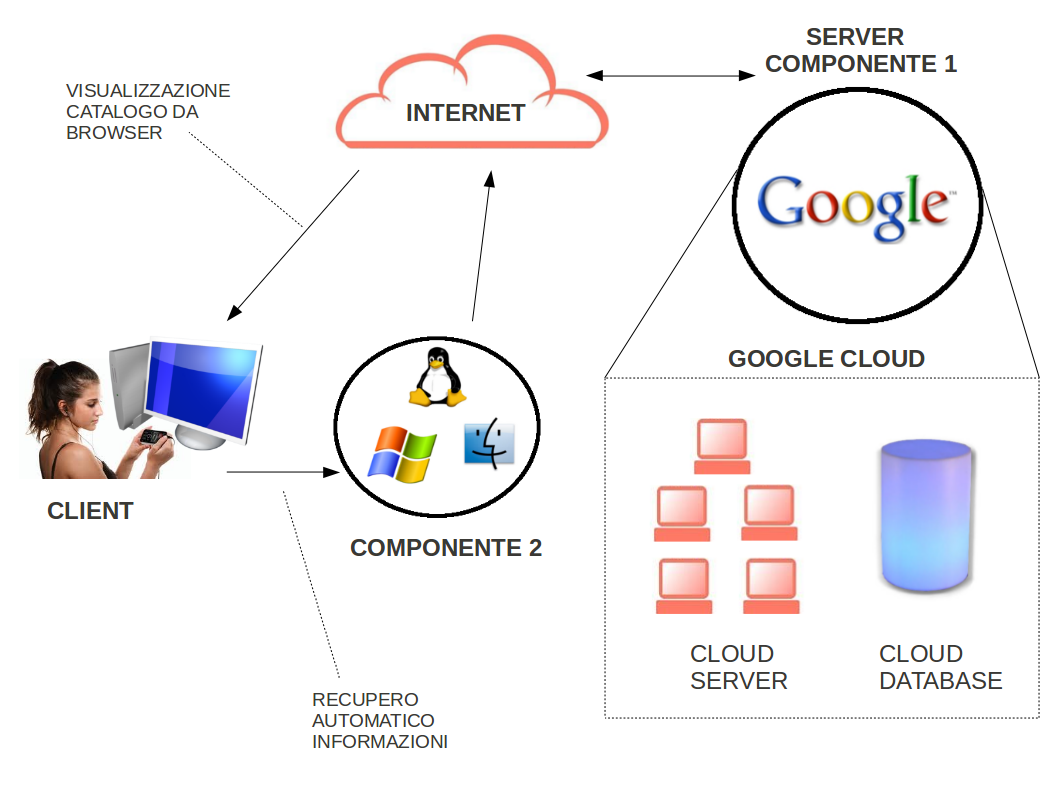
\includegraphics[width=16cm]{img/AR/DiagrammaArchitetturale.png}
\caption{Diagramma architetturale}
\end{figure}

\chapter{Use case}
\thispagestyle{fancy}

\section{UC1 - Sistema NetMus}

\begin{figure}[h]
  \centering
  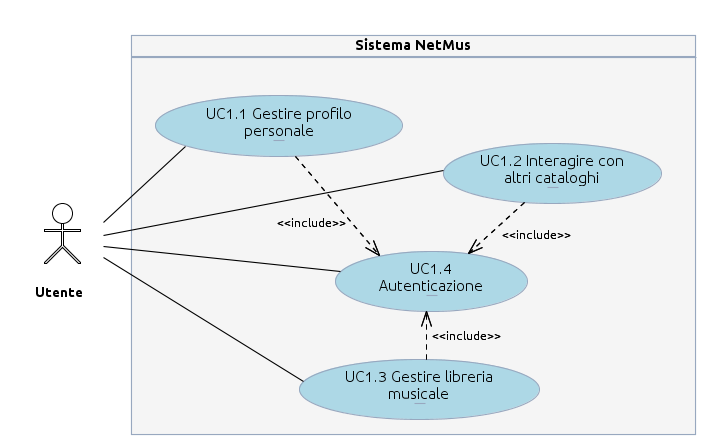
\includegraphics[width=18cm]{img/AR/UC1.png}
\caption{Diagramma UC1}
\end{figure}

\newpage
\vspace*{0.5cm}
\bo{Use case UC1: Sistema NetMus}\\\\
\bo{Attori primari: } Utente, Componente 1, Componente 2. \\\\
\bo{Pre-condizioni: } Entrambe le componenti sono attive e funzionanti, \`e
necessaria una connessione ad internet. \\\\ 
\bo{Post-condizioni: } La Componente 2 ha inviato al server tutte le
informazioni riguardanti nuovi brani musicali presenti nel computer o altre
periferiche dell'utente. La Componente 1 ha soddisfatto tutte le richieste
dell'utente. \\\\ 
\bo{Scenario principale: } 
\begin{enumerate}
  \item L'utente effettua l'autenticazione.
  \item Appena \`e attiva la connessione C2 invia le nuove informazioni al server.
  \item L'utente, tramite browser, fa un certo numero di richieste tra quelle
  possibili per visualizzare o modificare informazioni a C1.
  \item C1 soddisfa la richiesta dell'utente.
\end{enumerate}
\bo{Scenari secondari: }
\begin{itemize}
  \item La comunicazione tra utente e C1(server) fallisce per un problema di
  connessione.
  \begin {enumerate}
    \item Non c'\`e possibilit\`a di procedere fino a quando la connessione sar\`a
    ristabilita. I dati che erano stati aggiornati prima del verificarsi del
    problema sono gi\`a stati salvati.
  \end{enumerate}
  \item La comunicazione tra C2 e C1(server) fallisce per un problema di
  connessione.
  \begin {enumerate}
    \item C2 registra a che punto \`e arrivato l'invio e continua a lavorare in
    locale senza perdere informazioni.
  \end{enumerate}
\end{itemize}
\newpage


\section{UC1.1 - Sistema Netmus - Autenticazione}
\begin{figure}[h]
  \centering
  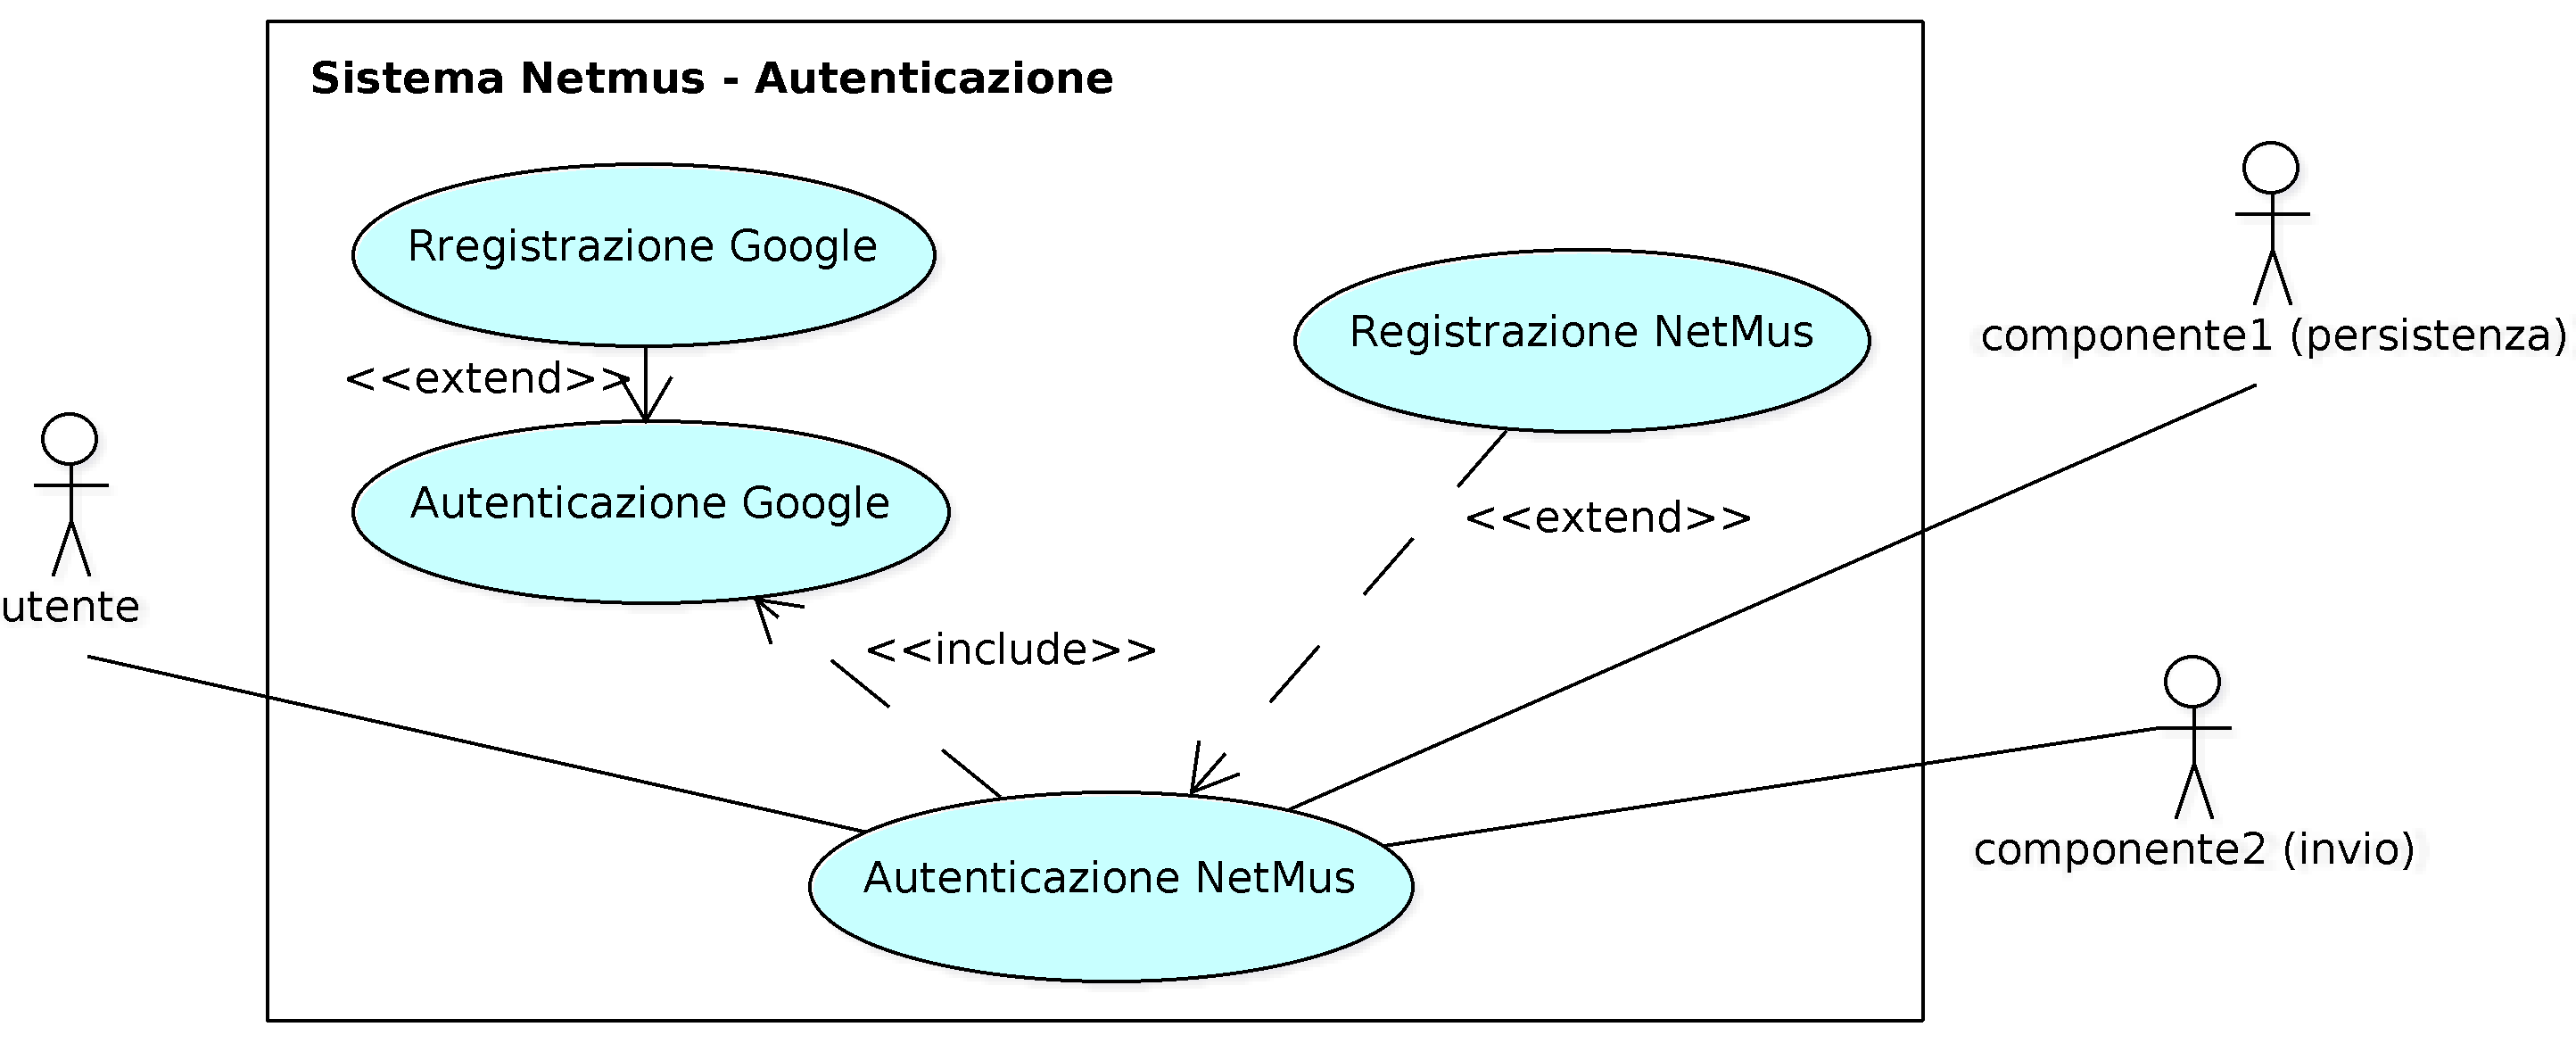
\includegraphics[width=15cm]{img/AR/UC1_1.png}
\caption{Diagramma UC1.1}
\end{figure}

\vspace{1cm}
\bo{Use case UC1.1: Sistema NetMus - Autenticazione}\\\\
\bo{Attori primari: } Utente, Componente 1, Componente 2. \\\\
\bo{Pre-condizioni: } Entrambe le componenti sono attive e funzionanti, \`e
necessaria una connessione ad internet. \\\\ 
\bo{Post-condizioni: } L'utente \`e autenticato all'interno del sistema NetMus. \\\\
\bo{Scenario principale: } 
\begin{enumerate}
  \item L'utente inserisce dei dati di login validi e se non li possiede
  li ottiene effettuando l'autenticazione/registrazione a Google e la
  registrazione a NetMus.
  \item Netmus verifica i dati ed autentica l'utente.
\end{enumerate}
\bo{Scenari secondari: }
\begin{itemize}
  \item L'utente inserisce dei dati di login non validi.
  \begin {enumerate}
    \item Il tentativo di autenticazione fallisce.
  \end{enumerate}
\end{itemize}
\newpage


\section{UC2 - Componente di persistenza e visualizzazione (C1)}
\begin{figure}[h]
  \centering
  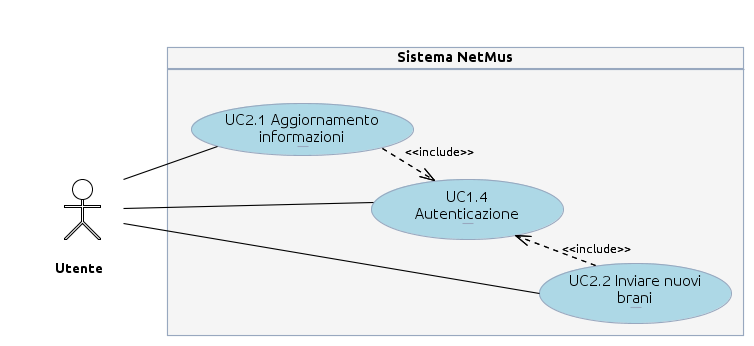
\includegraphics[width=16cm]{img/AR/UC2.png}
\caption{Diagramma UC2}
\end{figure}

\newpage
\vspace*{0.5cm}
\bo{Use case UC2: Componente di persistenza e visualizzazione (C1)}\\\\
\bo{Attori primari: } Utente, Google cloud (server + database). \\\\
\bo{Pre-condizioni: } L'utente ha aperto l'applicazione da browser ed \`e
autenticato. \\\\ 
\bo{Post-condizioni: } L'utente ha effettuato tutte le operazioni desiderate
con successo. \\\\
\bo{Scenario principale: } 
\begin{enumerate}
  \item L'utente naviga all'interno del proprio catalogo musicale presente nel
  database di NetMus, oppure all'interno di quello di un altro utente.
  \item L'utente seleziona le opzioni che preferisce, e fa alcune operazioni
  consentite.
  \item Tutti i dati richiesti dall'utente gli vengono forniti in tempo utile
  dal server (Google cloud).
\end{enumerate}
\bo{Scenari secondari: }
\begin{itemize}
  \item La comunicazione tra utente e server fallisce per un problema di
  connessione.
  \begin {enumerate}
    \item Non c'\`e possibilit\`a di procedere fino a quando la connessione sar\`a
    ristabilita. I dati che erano stati aggiornati prima del verificarsi del
    problema sono gi\`a stati salvati.
  \end{enumerate}
  \item L'utente cerca di accedere ad un altro profilo senza aver reso pubblico
  il proprio.
  \begin {enumerate}
    \item Viene chiesto all'utente se vuole pubblicare la propria libreria.
    \item In caso affermativo l'utente pu\`o procede a visualizzare altri profili,
    altrimenti gli viene negato l'accesso e viene rimandato alla propria pagina.
  \end{enumerate}
\end{itemize}
\newpage

\section{UC2.1 - C1 - Gestione catalogo}
\begin{figure}[h]
  \centering
  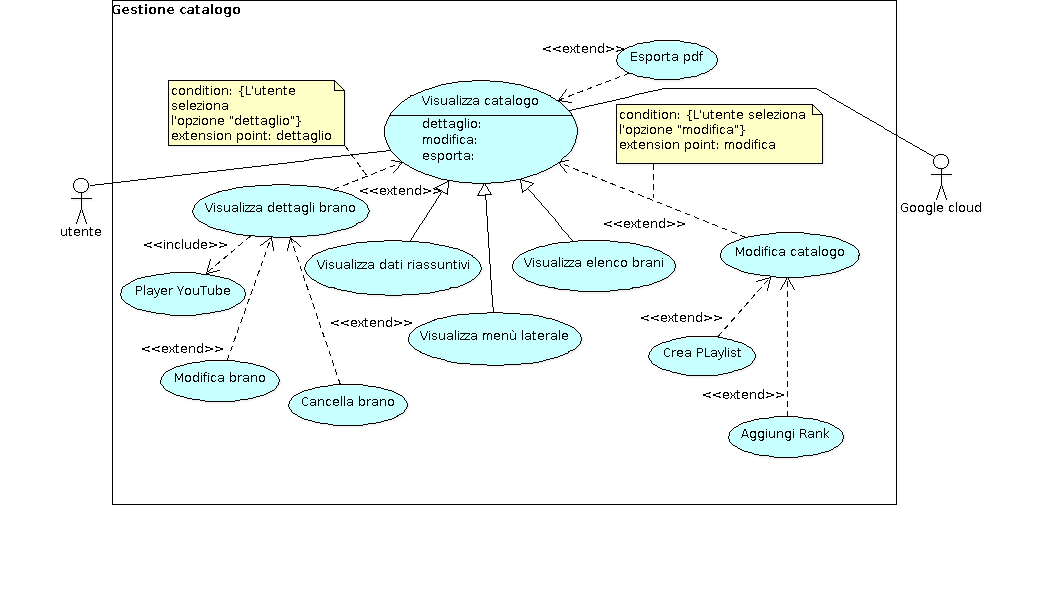
\includegraphics[width=18cm]{img/AR/UC2_1.png}
\caption{Diagramma UC2.1}
\end{figure}

\newpage
\vspace*{0.5cm}
\bo{Use case UC2.1: C1 - Gestione catalogo}\\\\
\bo{Attori primari: } Utente, Google cloud (server + database). \\\\
\bo{Pre-condizioni: } L'utente ha aperto l'applicazione da browser ed \`e
autenticato. \\\\ 
\bo{Post-condizioni: } L'utente \`e riuscito a vedere tutte le informazioni
salvate nella sua libreria musicale, sia quelle inviate dal suo computer sia
quelle aggiuntive recuperate dal database. L'utente ha inoltre
personalizzato il proprio catalogo a piacimento. \\\\
\bo{Scenario principale: } 
\begin{enumerate}
  \item L'utente visualizza la propria libreria di canzoni
  opportunamente raggruppate ed un men\`u sul lato sinistro per facilitare la
  navigazione all'interno della pagina, la visualizzazione \`e simile a quella
  del software \underline{iTunes}.
  \item L'utente seleziona il brano che gli interessa e ne visualizza i
  dettagli tra cui c'\`e anche il player di \underline{Youtube} che permette di ascoltare la
  canzone in streaming.
  \item In ogni momento, sia nella visualizzazione del catalogo sia in quella
  del singolo brano, l'utente pu\`o modificare varie opzioni e cancellare o
  aggiungere contenuti.
  \item Il server invia la pagina che l'utente ha richiesto e, se necessario,
  salva l'aggiornamento sui dati che ha fatto.
\end{enumerate}
\bo{Scenari secondari: }
\begin{itemize}
  \item La comunicazione tra utente e server fallisce per un problema di
  connessione.
  \begin {enumerate}
    \item Non c'\`e possibilit\`a di procedere fino a quando la connessione sar\`a
    ristabilita. I dati che erano stati aggiornati prima del verificarsi del
    problema sono gi\`a stati salvati.
  \end{enumerate}
  \item L'applicazione non ha trovato nessun corrispettivo del brano
  selezionato su YouTube.
  \begin {enumerate}
    \item Il player non viene visualizzato ma tutte le altre funzionalit\`a
    rimangono invariate.
  \end{enumerate}
\end{itemize}
\newpage


\section{UC2.2 - C1 - Elaborazione dati in entrata}
\begin{figure}[h]
  \centering
  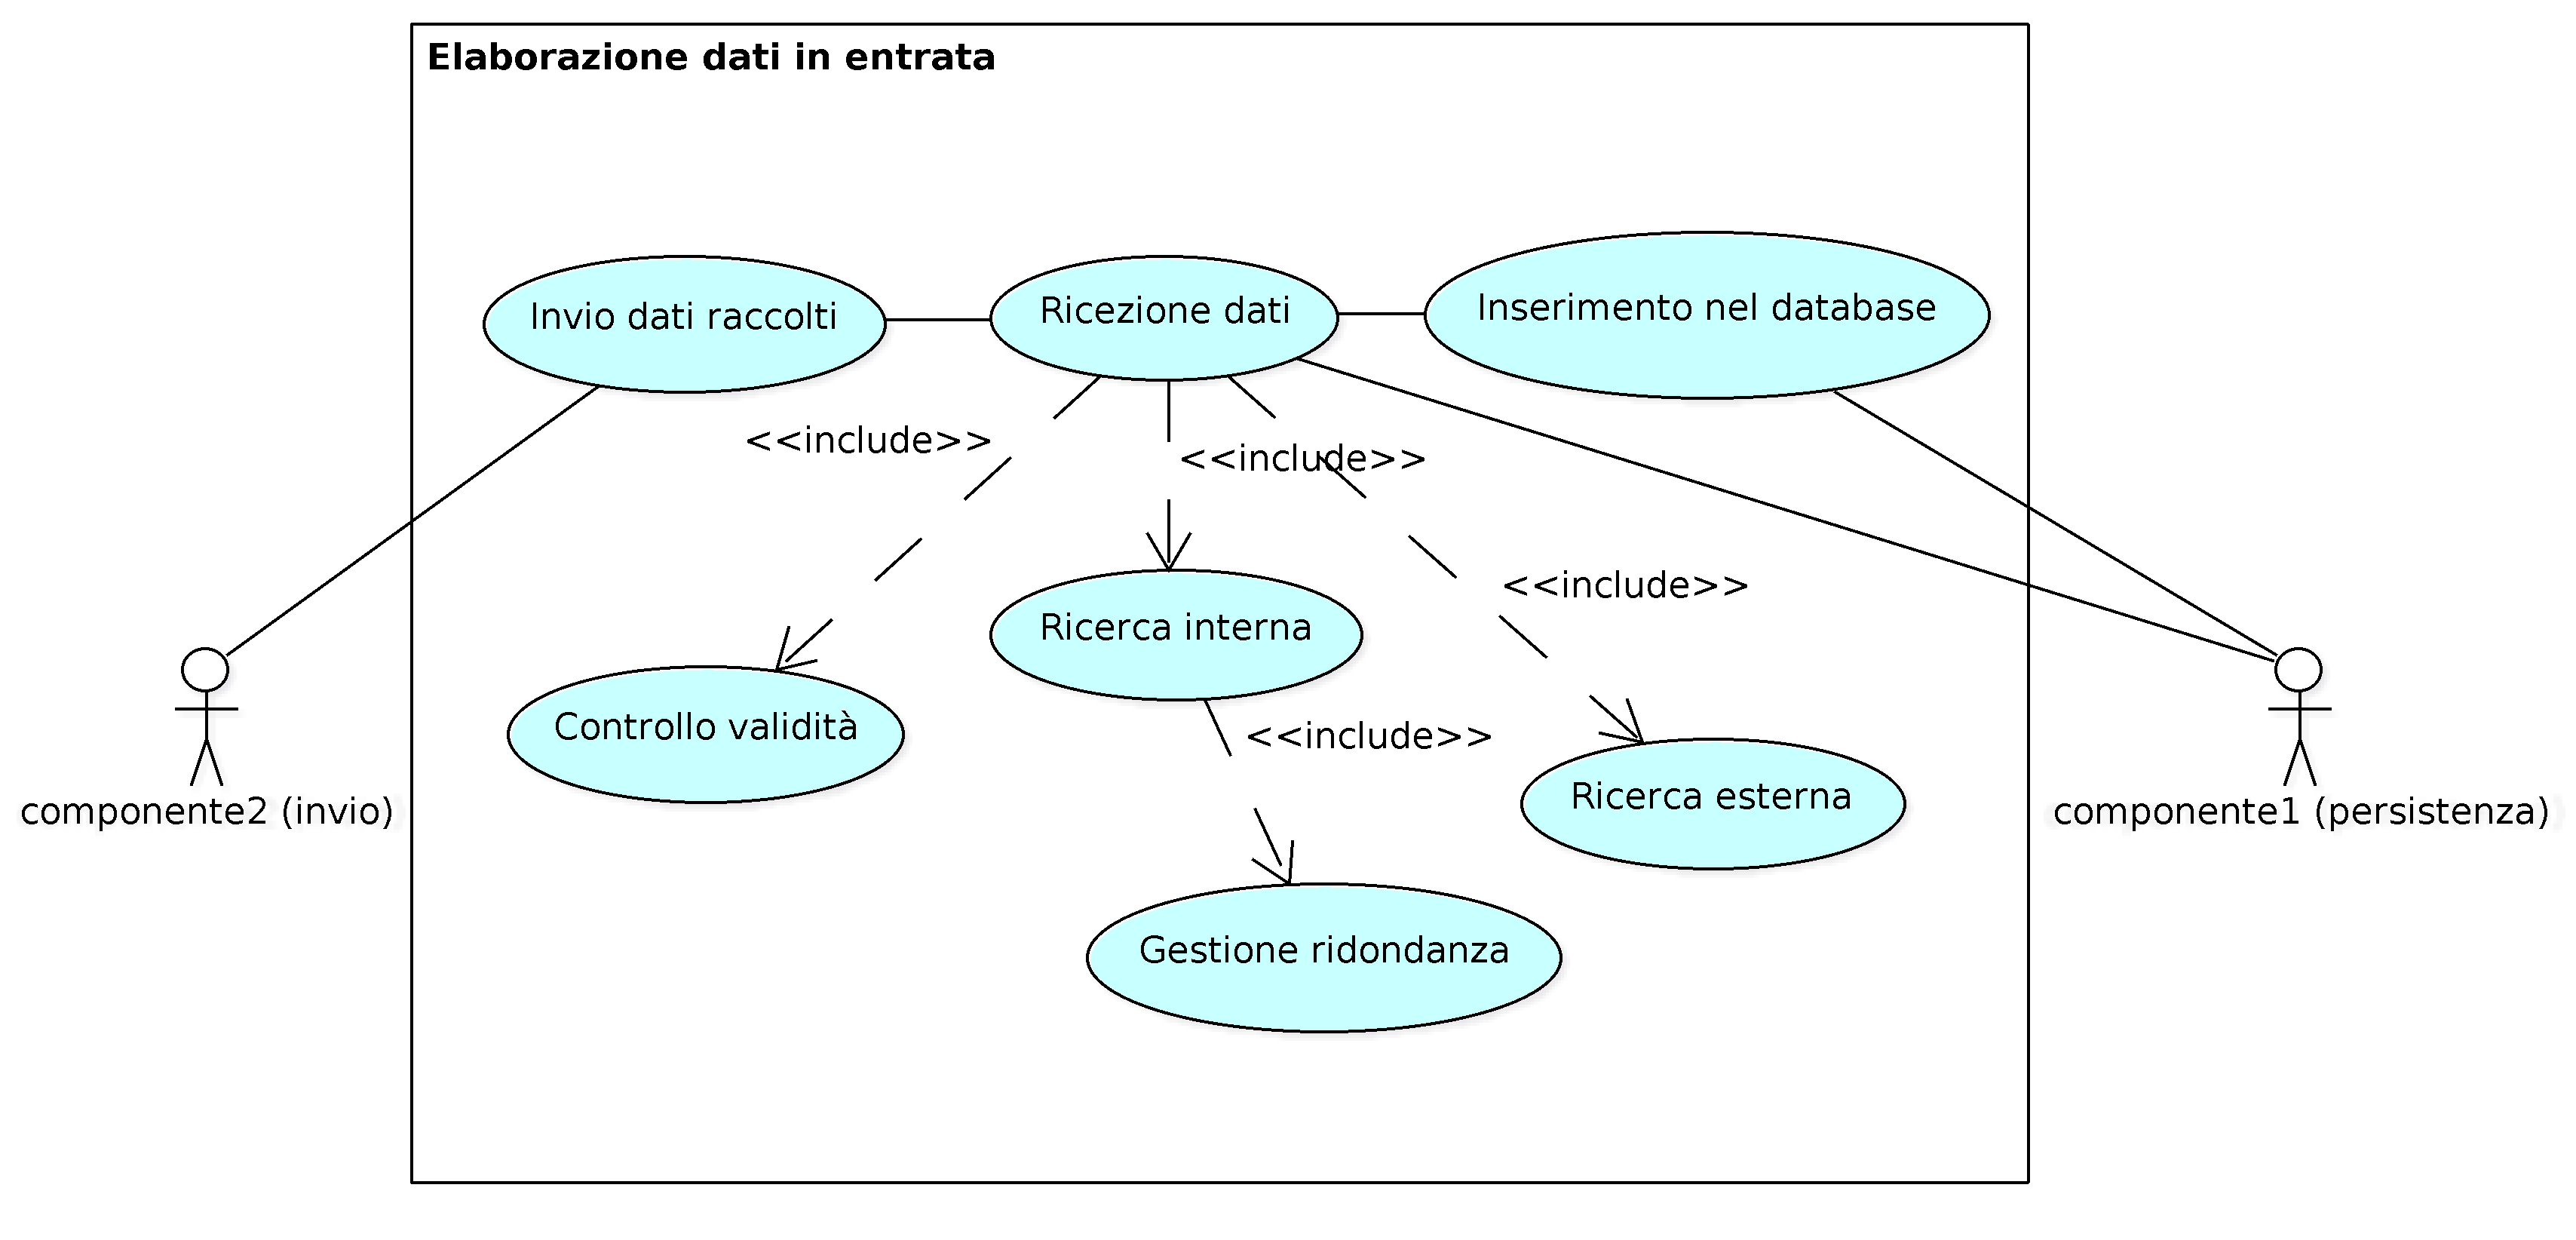
\includegraphics[width=18cm]{img/AR/UC2_2.png}
\caption{Diagramma UC2.2}
\end{figure}

\newpage
\vspace*{0.5cm}
\bo{Use case UC2.2: C1 - Elaborazione dati in entrata}\\\\
\bo{Attori primari: } Componente 2, Componente 1 (database). \\\\
\bo{Pre-condizioni: } Entrambe le componenti sono attive e funzionanti, la
componente di invio ha delle nuove informazioni da caricare, \`e necessaria una
connessione ad internet. \\\\ 
\bo{Post-condizioni: } Tutte le nuove informazioni valide sono state salvate
nel database insieme ad eventuali informazioni aggiuntive reperite da brani
preesistenti nel database oppure provenienti da un servizio esterno. \\\\
\bo{Scenario principale: } 
\begin{enumerate}
  \item C2 invia tutti i dati che ha raccolto.
  \item C1 controlla che non vi siano dati maligni o non riguardanti brani
  musicali.
  \item C1 effettua una ricerca nel proprio database per verificare se alcuni
  brani sono gi\`a presenti.
  \item C1 trova alcuni brani gi\`a in memoria e scarta i doppioni in entrata. Nel
  farlo, se le informazioni non combaciano precisamente, valuta quale delle due
  versioni \`e la pi\`u completa e adotta una strategia di ``\underline{merge}'' che minimizzi
  la ridondanza.
  \item Per i brani che non sono gi\`a presenti nel database C1 effettua una
  ricerca all'esterno e se trova informazioni aggiuntive per i brani in arrivo le inserisce.
  \item C1 salva i dati elaborati nel database.
\end{enumerate}
\bo{Scenari secondari: }
\begin{itemize}
  \item Vengono identificati alcuni dati maligni.
  \begin {enumerate}
    \item Queste informazioni vengono scartate senza possibilit\`a di ripristino e
    l'elaborazione procede senza conseguenze.
  \end{enumerate}
  \item C1 non riesce a stabilire se le informazioni relative a due brani
  descrivano effettivamente la stessa canzone.
  \begin {enumerate}
    \item Vengono tenuti entrambi i brani, fino a quando il sistema avr\`a
    abbastanza informazioni per decidere. L'elaborazione procede senza
    conseguenze.
  \end{enumerate}
\end{itemize}
\newpage

\section{UC3 - Componente di recupero delle informazioni (C2)}
\begin{figure}[h]
  \centering
  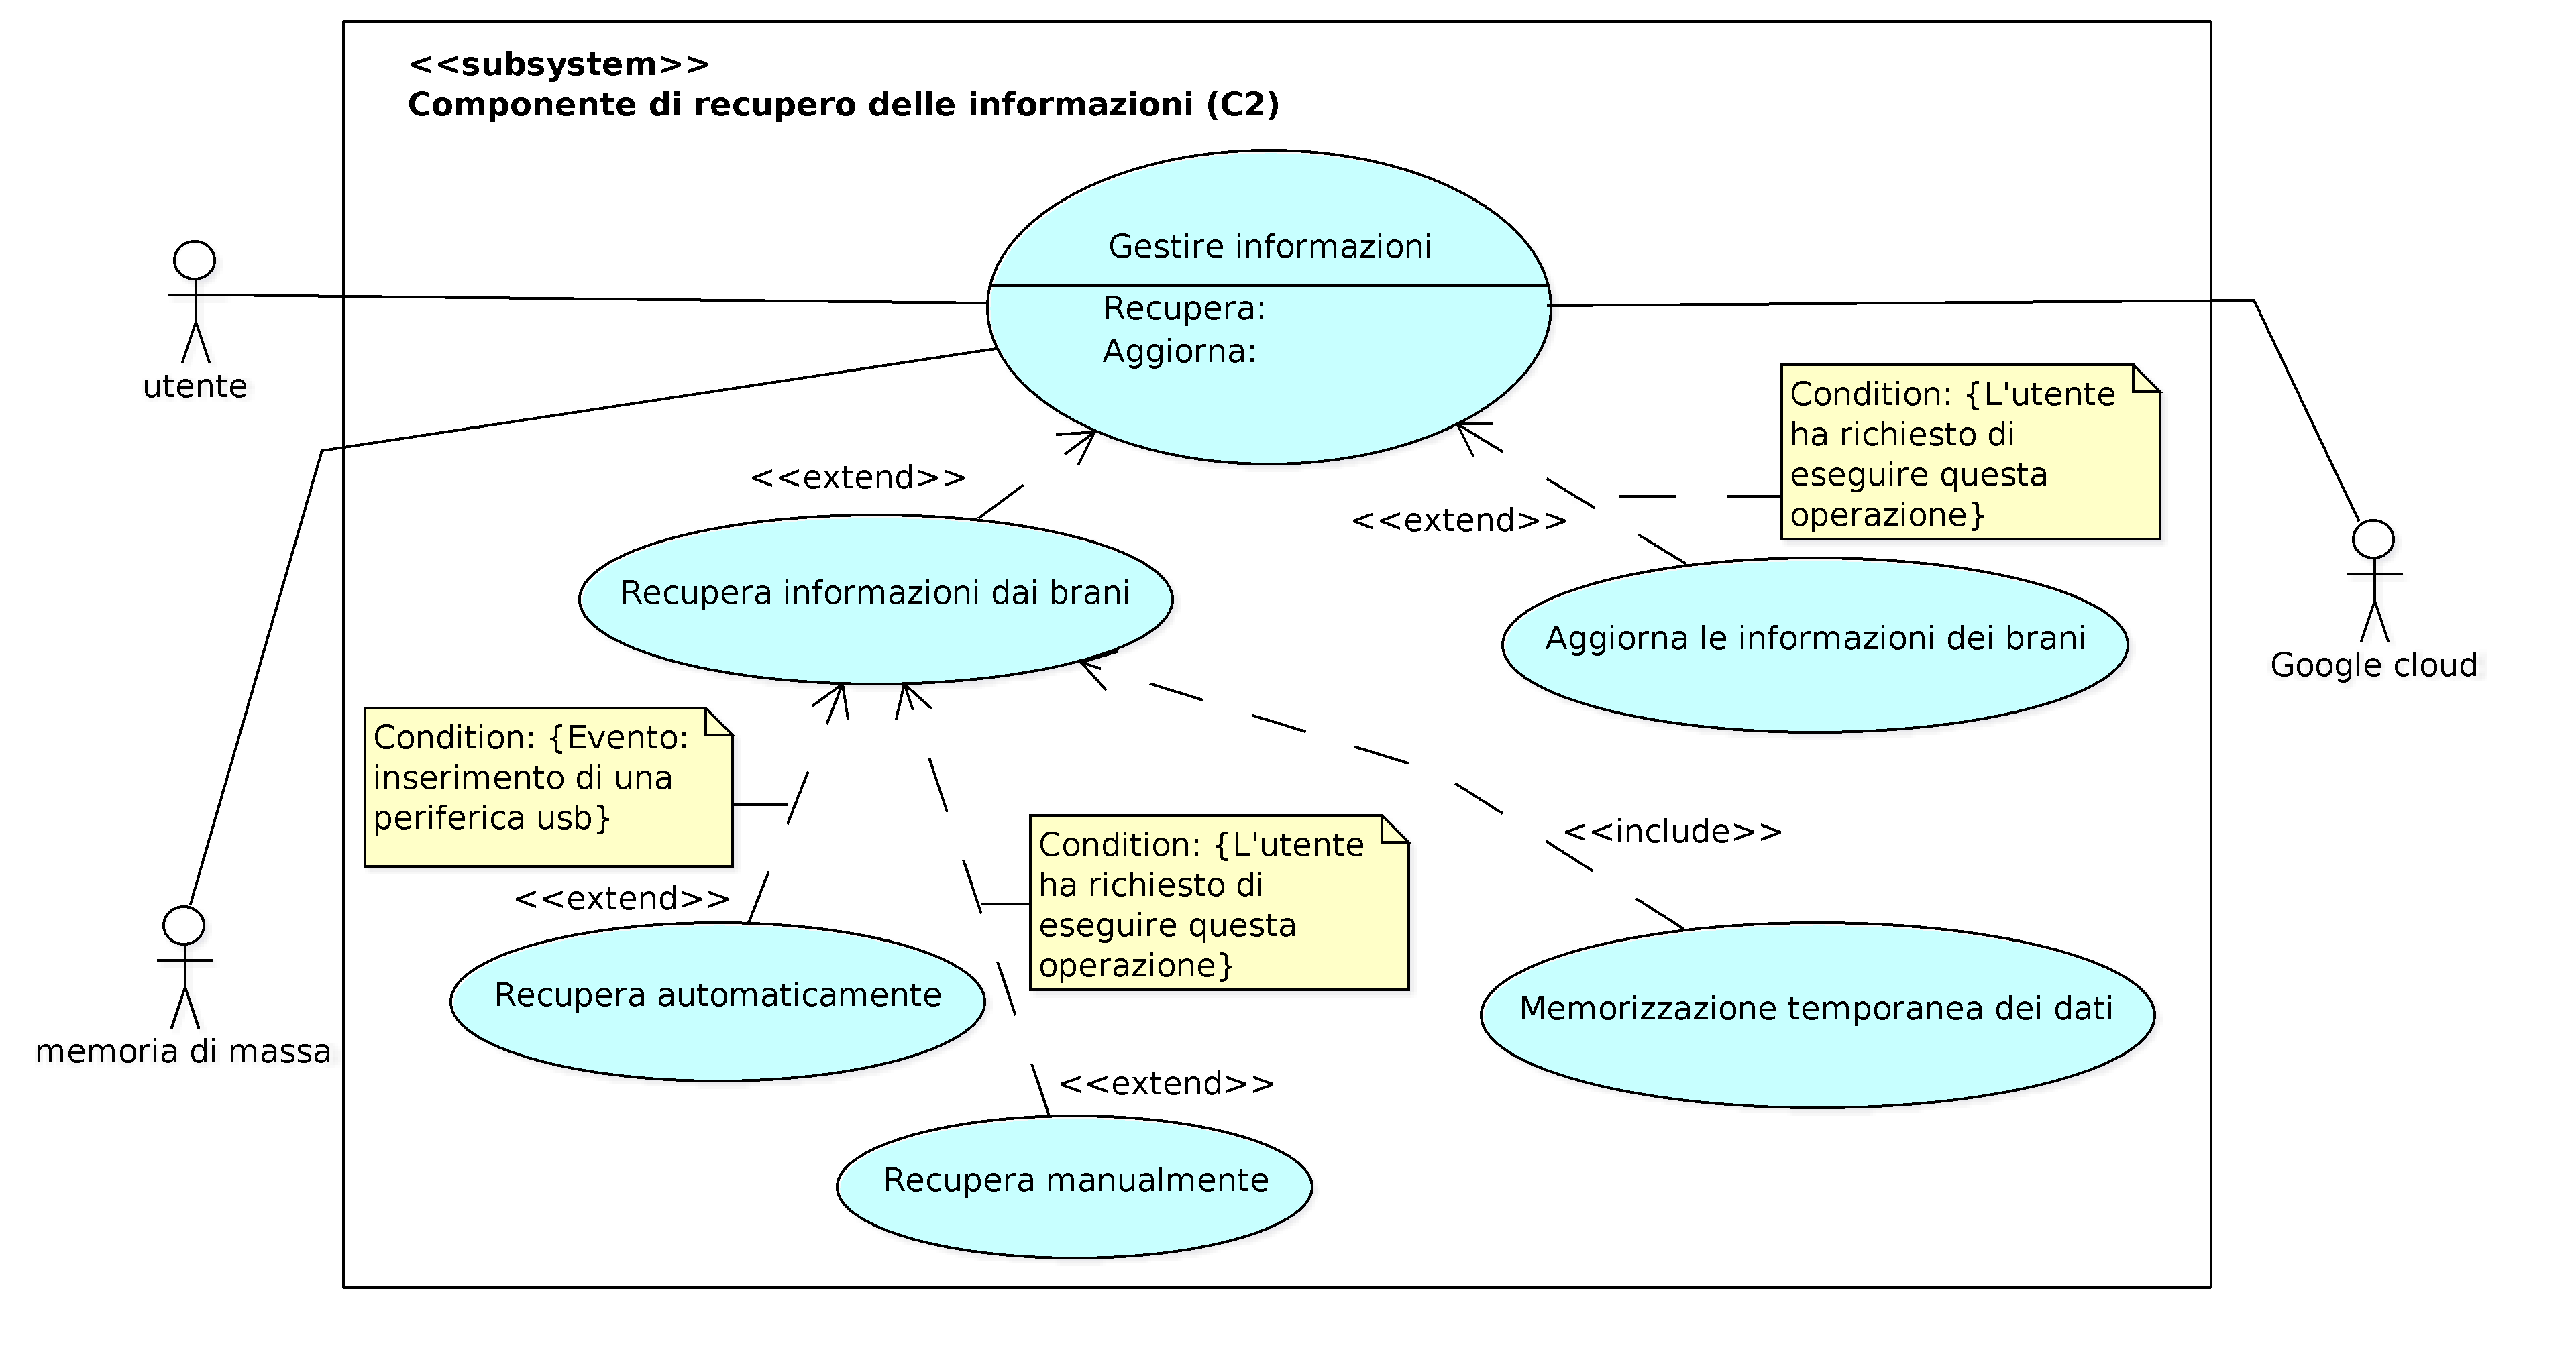
\includegraphics[width=16cm]{img/AR/UC3.png}
\caption{Diagramma UC3}
\end{figure}

\newpage
\vspace*{0.5cm}
\bo{Use case UC3: C2 - Recupero delle informazioni}\\\\
\bo{Attori primari: } Utente, Memoria di massa (intesa come hard disk e/o
periferiche usb), Google cloud. \\\\ \bo{Pre-condizioni: } La componente C2 \`e
attiva e funzionante, per alcune operazioni \`e necessaria la connessione ad internet \\\\
\bo{Post-condizioni: }
Gli eventuali nuovi brani individuati sono stati analizzati, e le relative
informazioni inviate a Google cloud.\\
Potrebbero essere stati aggiornati o completati i meta-dati dei brani. \\\\
\bo{Scenario principale: } \\
Raccolta dati:
\begin{enumerate}
  \item Viene inserita una nuova periferica usb, o avviata dall'utente una
  scansione manuale.
  \item C2 cerca tutti i brani.
  \item C2 estrapola le informazioni dei nuovi brani, scartando quelli senza
  informazioni, e le memorizza su un file temporaneo.
  \item C2 invia a Google cloud le informazioni dei nuovi brani.
  \item C2 elimina il file temporaneo.
\end{enumerate}
Aggiornamento dati:
\begin{enumerate}
  \item L'utente avvia l'aggiornamento delle informazioni dei brani.
  \item C2 invia a Google cloud la lista dei brani da aggiornare e/o completare.
  \item Google cloud invia a C2 le eventuali informazioni da aggiornare.
  \item C2 aggiorna le informazioni dei brani.
\end{enumerate}
\bo{Scenari secondari: }
\begin{itemize}
  \item Connessione non disponibile.
  \begin {enumerate}
    \item Per la raccolta dati, l'operazione procede senza conseguenze, e
    l'invio dei dati a Google cloud avverr\`a appena possibile in futuro.
    \item Per l'aggiornamento dei dati, l'elaborazione viene interrotta.
  \end{enumerate}
\end{itemize}
\newpage


\chapter{Lista dei requisiti}
\thispagestyle{fancy}
Ad ogni requisito \`e stato assegnato un codice di identificazione per facilitarne
il tracciamento, per maggiori informazioni per quanto riguarda la notazione
utilizzata per catalogare i requisiti si veda il documento
\emph{NormeDiProgetto-1.0.pdf}.

\section{Componente di persistenza e visualizzazione (C1)}
\subsection{Requisiti funzionali}

\subsubsection*{WEB Application NetMus}
\bo{Id:} C1FN-1 \\
\bo{Tipo:} funzionale \\
\bo{Richiesta:} obbligatorio \\
\bo{Fonte:} capitolato\\
La Componente 1 del software NetMus deve permettere la gestione di un catalogo
multimediale virtuale ad ogni utente che ha effettuato la registrazione.
Deve essere accessibile all'utente come \underline{applicazione WEB}.

\subsubsection*{Grafica simile ad iTunes}
\bo{Id:} C1FN-1.1 \\
\bo{Tipo:} funzionale \\
\bo{Richiesta:} obbligatorio \\
\bo{Fonte:} capitolato \\
L'interfaccia grafica deve dare un'esperienza di visualizzazione simile alla
libreria musicale fornita dal software iTunes (\url{http://www.apple.com/it/itunes/}).

\subsubsection*{Elenco brani}
\bo{Id:} C1FN-1.1.1 \\
\bo{Tipo:} funzionale \\
\bo{Richiesta:} obbligatorio \\
\bo{Fonte:} capitolato \\
La parte principale della visualizzazione della libreria \`e costituita
dall'elenco dei brani dell'utente opportunamente raggruppati e catalogati con la
possibilit\`a di ordinamento in base ad una o pi\`u delle categorie.

\subsubsection*{Menu laterali}
\bo{Id:} C1FN-1.1.2 \\
\bo{Tipo:} funzionale \\
\bo{Richiesta:} obbligatorio \\
\bo{Fonte:} capitolato \\
Come avviene in iTunes la navigazione tra le varie pagine deve essere favorita
da un comodo men\`u laterale alla sinistra della finestra dei brani.

\subsubsection*{Informazioni dettagliate brano}
\bo{Id:} C1FN-1.1.3 \\
\bo{Tipo:} funzionale \\
\bo{Richiesta:} obbligatorio \\
\bo{Fonte:} capitolato \\
Per ognuno dei propri brani catalogati sar\`a possibile accedere alle informazioni
dettagliate, come ad esempio la copertina dell'album, in una nuova finestra

\subsubsection*{Player YouTube}
\bo{Id:} C1FD-1.1.4 \\
\bo{Tipo:} funzionale \\
\bo{Richiesta:} desiderabile \\
\bo{Fonte:} capitolato \\
Insieme alle informazioni di un brano dovrebbe comparire anche un player fornito
da Youtube con cui ascoltarlo.

\subsubsection*{Registrazione}
\bo{Id:} C1FN-1.2 \\
\bo{Tipo:} funzionale \\
\bo{Richiesta:} obbligatorio \\
\bo{Fonte:} capitolato \\
Un individuo pu\`o diventare utente di Netmus ed avere la possibilit\`a di gestire
il proprio catalogo multimediale solamente dopo aver effettuato la
registrazione, che prevede l'inserimento di un \underline{username} (unico), una
password ed un indirizzo email (attraverso cui fare la conferma) pi\`u alcune
informazioni personali.

\subsubsection*{Pagina di login}
\bo{Id:} C1FN-1.2.1 \\
\bo{Tipo:} funzionale \\
\bo{Richiesta:} obbligatorio \\
\bo{Fonte:} verbale1 \\
L'applicazione avr\`a un sistema di autenticazione proprio oltre a fornire
l'autenticazione di Google acquisita da \underline{Google AppEngine}.

\subsubsection*{Personalizzazione catalogo}
\bo{Id:} C1FN-1.3 \\
\bo{Tipo:} funzionale \\
\bo{Richiesta:} obbligatorio \\
\bo{Fonte:} interna \\
La gestione del catalogo prevede alcuni metodi di personalizzazione basilari che
permettono all'utente di visualizzare la propria libreria nel modo preferito ma
che non vanno a modificare le informazioni a livello di database.

\subsubsection*{Cancellazione brano}
\bo{Id:} C1FN-1.3.1 \\
\bo{Tipo:} funzionale \\
\bo{Richiesta:} obbligatorio \\
\bo{Fonte:} verbale1 \\
Un utente potr\`a rimuovere dalla propria libreria qualche brano, i dati
rimarranno nel database.

\subsubsection*{Modifica informazioni brano}
\bo{Id:} C1FD-1.3.2 \\
\bo{Tipo:} funzionale \\
\bo{Richiesta:} desiderabile \\
\bo{Fonte:} interna \\
Tutte le informazioni di un brano potranno essere modificate dall'utente che le
ha caricate, il database non risentir\`a di questi cambiamenti quindi gli altri
utenti non risentiranno in alcun modo di questi cambiamenti.

\subsubsection*{Creazione playlist}
\bo{Id:} C1FO-1.3.3 \\
\bo{Tipo:} funzionale \\
\bo{Richiesta:} opzionale \\
\bo{Fonte:} interna \\
Viene data all'utente la possibilit\`a di creare delle liste lunghe a piacere dei
propri brani allo scopo di ordinare la propria libreria oppure di ascoltarle in
sequenza attraverso i player.

\subsubsection*{Ranking brani}
\bo{Id:} C1FO-1.3.4 \\
\bo{Tipo:} funzionale \\
\bo{Richiesta:} opzionale \\
\bo{Fonte:} interna \\
L'utente pu\`o assegnare un punteggio ad ogni brano in base al suo gradimento
personale, questo pu\`o tornare utile come criterio di ordinamento.

\subsubsection*{Gestione profilo personale}
\bo{Id:} C1FN-1.4 \\
\bo{Tipo:} funzionale \\
\bo{Richiesta:} obbligatorio \\
\bo{Fonte:} interna \\
In ogni momento l'utente di NetMus pi\`u modificare i suoi dati di registrazione,
eccetto l'username. Il profilo, se desiderato, pu\`o diventare pubblico e visibile
dagli altri utenti fornendo la possibilit\`a di confrontare il proprio catalogo
musicale e le le altre informazioni.

\subsubsection*{Modifica informazioni personali}
\bo{Id:} C1FN-1.4.1 \\
\bo{Tipo:} funzionale \\
\bo{Richiesta:} obbligatorio \\
\bo{Fonte:} interna \\
Una volta effettuato il login sar\`a possibile accedere ad una pagina apposita per
aggiornare ed aggiungere informazioni al proprio profilo.

\subsubsection*{Cambio password}
\bo{Id:} C1FN-1.4.2 \\
\bo{Tipo:} funzionale \\
\bo{Richiesta:} obbligatorio \\
\bo{Fonte:} interna \\
Quando l'utente lo desidera pu\`o cambiare la password del proprio account.

\subsubsection*{Cancellazione account}
\bo{Id:} C1FN-1.4.3 \\
\bo{Tipo:} funzionale \\
\bo{Richiesta:} obbligatorio \\
\bo{Fonte:} interna \\
Deve essere possibile per ogni utente chiudere il proprio profilo in maniera
permanente eliminando dal database ogni sua informazione.

\subsubsection*{Pubblicazione profilo}
\bo{Id:} C1FD-1.4.4 \\
\bo{Tipo:} funzionale \\
\bo{Richiesta:} desiderabile \\
\bo{Fonte:} interna \\
Per interagire con gli altri sar\`a necessario pubblicare il proprio profilo e
di conseguenza la propria libreria di canzoni rendendo visibile a tutti ci\`o che
contengono.

\subsubsection*{Riproduzione tracce in streaming}
\bo{Id:} C1FD-1.5 \\
\bo{Tipo:} funzionale \\
\bo{Richiesta:} desiderabile \\
\bo{Fonte:} capitolato \\
NetMus prevede un sistema di riproduzione delle canzoni salvate nel database.
Non contenendo alcun file multimediale l'ascolto sar\`a reso possibile dalla
riproduzione in streaming fornita da Youtube. La ricerca dei brani
corrispondenti alle informazioni nel database sar\`a a totale carico
dell'applicazione NetMus.

\subsubsection*{Interazione con altri utenti}
\bo{Id:} C1FD-1.7 \\
\bo{Tipo:} funzionale \\
\bo{Richiesta:} desiderabile \\
\bo{Fonte:} interna \\
La comunicazione con altri utenti sar\`a favorita da alcune semplici funzionalit\`a
che rendono la propria libreria oggetto di confronto dando pi\`u spazio
allo scambio di idee e conoscenze tra gli utilizzatori di NetMus.

\subsubsection*{Visualizzazione altri profili}
\bo{Id:} C1FD-1.7.1 \\
\bo{Tipo:} funzionale \\
\bo{Richiesta:} desiderabile \\
\bo{Fonte:} interna \\
Sar\`a possibile visualizzare l'intera libreria musicale e le altre informazioni
di tutti gli utenti che hanno permesso la condivisione del proprio profilo.

\subsubsection*{Lasciare commenti}
\bo{Id:} C1FO-1.7.2 \\
\bo{Tipo:} funzionale \\
\bo{Richiesta:} opzionale \\
\bo{Fonte:} interna \\
Uno strumento semplice ma molto coinvolgente sar\`a la possibilit\`a di scrivere
commenti alle informazioni condivise da altri utenti come brani, autori e
playlist.

\subsubsection*{Elaborazione dati utente}
\bo{Id:} C1FD-1.8 \\
\bo{Tipo:} funzionale \\
\bo{Richiesta:} desiderabile \\
\bo{Fonte:} interna \\
Il sistema NetMus si occuper\`a anche di elaborare in modo intelligente i dati
raccolti dai vari utenti permettendo di avere nel proprio profilo dei dati
riassuntivi riguardanti la propria libreria ma anche di avere delle informazioni
di confronto con le librerie degli altri utenti.

\subsubsection*{Esportazione pdf}
\bo{Id:} C1FO-1.8.1 \\
\bo{Tipo:} funzionale \\
\bo{Richiesta:} opzionale \\
\bo{Fonte:} interna \\
Sar\`a possibile esportare il proprio catalogo opportunamente indicizzato e con
informazioni aggiuntive procurate da NetMus in formato \underline{pdf}
predisposto per la stampa.

\subsubsection*{Ricezione ed elaborazione brani}
\bo{Id:} C1FN-1.9 \\
\bo{Tipo:} funzionale \\
\bo{Richiesta:} obbligatorio \\
\bo{Fonte:} capitolato \\
Netmus deve occuparsi della rizeione dei dati in arrivo da tutte le componenti
di invio che si connettono ad esso, dovr\`a quindi gestire queste connessioni in
modo concorrente nel miglior modo possibile. Inoltre per tutte le informzioni
ricevute con successo si occuper\`a di verificarne la validit\`a e di arricchirne i
contenuti ove possibile.

\subsubsection*{Controllo validit\`a dati}
\bo{Id:} C1FN-1.9.1 \\
\bo{Tipo:} funzionale \\
\bo{Richiesta:} obbligatorio \\
\bo{Fonte:} capitolato \\
Tutte le informazioni inviate da C2 saranno controllate in maniera
rapida ma che garantisca che non vi siano dati maligni per NetMus o che non
riguardino brani musicali.

\subsubsection*{Completamento informazioni da database interno}
\bo{Id:} C1FN-1.9.2 \\
\bo{Tipo:} funzionale \\
\bo{Richiesta:} obbligatorio \\
\bo{Fonte:} interna \\
Sar\`a sfruttato il database interno per completare ed aggiungere informazioni
mancanti ai brani in entrata. Questo sar\`a fatto basandosi su opportuni algoritmi
di ricerca che garantiscano un buona probabilit\`a che i dati suggeriti per
l'aggiornamento siano quelli corretti.

\subsubsection*{Inserimento nel database}
\bo{Id:} C1FN-1.9.5 \\
\bo{Tipo:} funzionale \\
\bo{Richiesta:} obbligatorio \\
\bo{Fonte:} capitolato \\
Una volta controllate ed aggiornate le informazioni ricevute verranno salvate
nel database entrando a far parte a tutti gli effetti della libreria musicale
dell'utente da cui sono state ricevute.

\subsubsection*{Completamento informazioni da servizio esterno}
\bo{Id:} C1FO-1.9.3 \\
\bo{Tipo:} funzionale \\
\bo{Richiesta:} opzionale \\
\bo{Fonte:} capitolato \\
Per reperire informazioni sicure che possano servire per correggere eventuali
dati mancanti riguardo i brani inviati a NetMus, se il database interno non le
possiede, si sfrutter\`a uno o pi\`u servizi gratuiti esterni.

\subsubsection*{Invio nuove informazioni a C2}
\bo{Id:} C1FD-1.10 \\
\bo{Tipo:} funzionale \\
\bo{Richiesta:} desiderabile \\
\bo{Fonte:} verbale1 \\
Se saranno trovate informazioni aggiuntive, da database interno o esterno, ai
dati inviati da qualche utente sar\`a possibile anche, se desiderato, inviarle
a C2 per andare ad aggiornare i file multimediali dell'utente.

\subsubsection*{Gestione database}
\bo{Id:} C1FN-1.13 \\
\bo{Tipo:} funzionale \\
\bo{Richiesta:} obbligatorio \\
\bo{Fonte:} capitolato \\
Il fulcro della persistenza del sistema NetMus sar\`a un database nel quale
verranno salvati tutti i dati gestiti. In particolare il database sar\`a quello
fornito da Google AppEngine, Google DataStore che trae grandissimi benefici dal
\underline{cloud computing}.

\subsection{Requisiti di qualit\`a}

\subsubsection*{Ottimizzazione della ricerca su YoutTube}
\bo{Id:} C1QD-1.5.1 \\
\bo{Tipo:} qualit\`a \\
\bo{Richiesta:} desiderabile \\
\bo{Fonte:} interna \\
Youtube \`e uno strumento estremamente utile poich\'e garantisce una vasta gamma di
dati sulla quale fare ricerche ma proprio per questo sar\`a importante che NetMus
implementi degli algoritmi opportuni che eseguano queste ricerche in modo molto
efficiente.

\subsubsection*{Identificazione dati ridondanti}
\bo{Id:} C1QN-1.9.4 \\
\bo{Tipo:} qualit\`a \\
\bo{Richiesta:} obbligatorio \\
\bo{Fonte:} interna \\
NetMus sar\`a in grado di associare le informazioni simili e
riguardanti lo stesso brano in modo da inserirle una sola vola all'interno del
database. Questo verr\`a fatto solo se si ha la sicurezza che si tratti dello
stesso brano, altrimenti verranno mantenute le diverse versioni fino a quando si
avranno informazioni sufficienti per saperlo.

\subsubsection*{Gestione concorrenza}
\bo{Id:} C1QN-1.9.6 \\
\bo{Tipo:} qualit\`a \\
\bo{Richiesta:} obbligatorio \\
\bo{Fonte:} interna \\
La componente di persistenza sar\`a in grado di gestire la concorrenza tra le
richieste di invio dati simultanee da vari clients in modo da garantire una
corretta ricezione di tutte le informazioni.

\subsubsection*{Scalabilit\`a}
\bo{Id:} C1QN-1.6 \\
\bo{Tipo:} qualit\`a \\
\bo{Richiesta:} obbligatorio \\
\bo{Fonte:} capitolato \\
NetMus garantir\`a la possibilit\`a di crescere di dimensione, in tutti i vari
aspetti, senza dover effettuare alcun ritocco o modifica all'architettura del
sistema.

\subsubsection*{Scalabilit\`a interfaccia grafica}
\bo{Id:} C1QN-1.6.1 \\
\bo{Tipo:} qualit\`a \\
\bo{Richiesta:} obbligatorio \\
\bo{Fonte:} capitolato \\
La libreria personale dell'utente sar\`a potenzialmente infinita, di conseguenza
le pagine che ne permetteranno la visualizzazione saranno in grado di adattarsi
senza imporre vincoli di alcun tipo.

\subsubsection*{Scalabilit\`a massa di utenza}
\bo{Id:} C1QN-1.6.2 \\
\bo{Tipo:} qualit\`a \\
\bo{Richiesta:} obbligatorio \\
\bo{Fonte:} capitolato \\
Poich\'e il bacino d'utenza potenziale \`e estremamente elevato NetMus sar\`a molto
efficiente per quanto riguarda gli accessi simultanei di molti utenti
all'\underline{applicazione web}ed al database.

\subsubsection*{Cloud computing}
\bo{Id:} C1QN-1.11 \\
\bo{Tipo:} qualit\`a \\
\bo{Richiesta:} obbligatorio \\
\bo{Fonte:} capitolato \\
Sar\`a utilizzato il supporto al cloud computing fornito da Google AppEngine,
anche per quanto riguarda il database grazie a Google DataStore.

\subsubsection*{Utilizzo}
\bo{Id:} C1QN-2 \\
\bo{Tipo:} qualit\`a \\
\bo{Richiesta:} obbligatorio \\
\bo{Fonte:} interna \\
Un occhio di riguardo sar\`a dato alla semplicit\`a di utilizzo ed alla possibilit\`a
per tutti i potenziali utenti di imparare ad utilizzare NetMus. L'utente
deve poter essere subito in grado di visualizzare e gestire il proprio catalogo
musicale dopo essersi registrato ed aver messo in funzione la C2.

\subsubsection*{Accessibilit\`a}
\bo{Id:} C1QO-2.1 \\
\bo{Tipo:} qualit\`a \\
\bo{Richiesta:} opzionale \\
\bo{Fonte:} interna \\
Il software Web presenter\`a alcune caratteristiche per favorire l'accesso a
qualsiasi tipologia di utenza come ad esempio il \underline{codice sorgente}
validato secondo parametri \underline{W3C}.

\subsubsection*{Portabilit\`a}
\bo{Id:} C1QN-2.3 \\
\bo{Tipo:} qualit\`a \\
\bo{Richiesta:} obbligatorio \\
\bo{Fonte:} interna \\
Deve essere compatibile col maggior numero di configurazioni software e
hardware.

\subsubsection*{Supporto multi-lingua}
\bo{Id:} C1QD-2.4 \\
\bo{Tipo:} qualit\`a \\
\bo{Richiesta:} desiderabile \\
\bo{Fonte:} capitolato \\
Saranno accessibili due versioni dell'applicazione, una in italiano ed una in
lingua inglese, con gli stessi contenuti e sar\`a possibile spostarsi da una
all'altra in qualsiasi momento.

\subsubsection*{Manutenibilit\`a}
\bo{Id:} C1QN-2.6 \\
\bo{Tipo:} qualit\`a \\
\bo{Richiesta:} obbligatorio \\
\bo{Fonte:} interna \\
Saranno seguiti dei criteri di scrittura del codice e stesura dei documenti che
favoriranno il pi\`u possibile il processo di manutenzione.

\subsubsection*{Gestione errori}
\bo{Id:} C1QN-2.7 \\
\bo{Tipo:} qualit\`a \\
\bo{Richiesta:} obbligatorio \\
\bo{Fonte:} interna \\
Il sistema sar\`a robusto relativamente agli errori causati all'utilizzo della
rete internet, notoriamente inaffidabile.

\subsubsection*{Manuale utente}
\bo{Id:} C1QN-3.1 \\
\bo{Tipo:} qualit\`a \\
\bo{Richiesta:} obbligatorio \\
\bo{Fonte:} capitolato \\
Sar\`a redatto un manuale utente che conterr\`a tutte e sole le informazioni
necessarie all'utilizzo di NetMus in modo da essere facilmente comprensibile da
tutta l'enorme fascia di utenza a cui si rivolge.

\subsubsection*{Manuale utente inglese}
\bo{Id:} C1QD-3.1.1 \\
\bo{Tipo:} qualit\`a \\
\bo{Richiesta:} desiderabile \\
\bo{Fonte:} capitolato \\
Sar\`a fornita anche una traduzione del manuale utente in lingua inglese.


\subsection{Requisiti di vincolo}

\subsubsection{Interfacciamento con gli ambienti di installazione e d'uso }

\subsubsection*{Tecnologie GAE e GWT}
\bo{Id:} C1VN-1.12 \\
\bo{Tipo:} vincolo \\
\bo{Richiesta:} obbligatorio \\
\bo{Fonte:} capitolato \\
Per lo sviluppo dell'applicazione Web NetMus sar\`a utilizzata la piattaforma
\underline{Google AppEngine (GAE)} in concomitanza con l'insieme di strumenti
forniti da \underline{Google Web Toolkit (GWT)}. Entrambi sono gratuiti.

\subsubsection*{Google DataStore}
\bo{Id:} C1VN-1.13.1 \\
\bo{Tipo:} vincolo \\
\bo{Richiesta:} obbligatorio \\
\bo{Fonte:} capitolato \\
Il database verr\`a sviluppato utilizzando \underline{Google DataStore}.

\subsubsection{Norme vigenti nel dominio applicativo}

\subsubsection*{Quote YouTube}
\bo{Id:} C1VD-1.5.2 \\
\bo{Tipo:} vincolo \\
\bo{Richiesta:} desiderabile \\
\bo{Fonte:} interna \\
NetMus rispetter\`a le quote di traffico imposte da Youtube per quanto riguarda
il traffico in entrata ed in uscita dai loro server.

\subsubsection*{YouTube Terms of Service}
\bo{Id:} C1VD-1.5.3 \\
\bo{Tipo:} vincolo \\
\bo{Richiesta:} desiderabile \\
\bo{Fonte:} interna \\
NetMus rispetter\`a le regole stabilite da YouTube per quanto riguarda i\\
propri contenuti (\url{http://www.youtube.com/t/terms}) e per quanto
riguarda l'utilizzo delle YouTube API
(\url{http://code.google.com/apis/youtube/terms.html}).

\subsubsection*{Open source}
\bo{Id:} C1VN-2.2 \\
\bo{Tipo:} vincolo \\
\bo{Richiesta:} obbligatorio \\
\bo{Fonte:} capitolato \\
La licenza d'uso dell'applicazione sar\`a di tipo \underline{Open source}.

\subsubsection{Caratteristiche dell'utente}

\subsubsection*{Semplicit\`a di utilizzo}
\bo{Id:} C1VN-2.5 \\
\bo{Tipo:} vincolo \\
\bo{Richiesta:} obbligatorio \\
\bo{Fonte:} interna \\
Tutte le componenti dell'applicazione Web NetMus saranno mirate alla semplicit\`a
di utilizzo da parte dell'utente. A partire dall'interfaccia grafica sar\`a tutto
molto intuitivo.


\subsection{Gerarchia dei requisiti}

\begin{table}[!h]
\centering
\begin{footnotesize}
\begin{tabular}{|l|l|}

\rowcolor{Orange}
\bo{Web Application Netmus} \\
\hline
\cellcolor{orange}
Grafica simile ad iTunes & Elenco brani raggruppati opportunamente \\
& Menu laterali \\   
& Visualizzazione informazioni dettagliate di un brano \\         
& Visualizza player youtube \\         
\hline
\cellcolor{orange}
Creazione profilo utente tramite registrazione & Pagina di login dipendente da Google login \\ 
\hline
\cellcolor{orange}
Personalizzazione del proprio catalogo & Cancellazione brano \\
& Modifica informazioni brano \\       
& Creazione playlist \\
& Ranking brani \\   
\hline
\cellcolor{orange}
Gestione profilo personale & Modifica informazioni personali \\         
& Cambio password \\
& Cancellazione del proprio account \\       
& Publicazione profilo \\
\hline
\cellcolor{orange}
Riproduzione tracce in streaming & Ottimizzazione della ricerca su Youtube \\       
& Quote Youtube \\
& Youtube Terms of Service \\       
\hline
\cellcolor{orange}
Scalabilit\`a & Scalabilit\`a di interfaccia grafica \\       
& Scalabilit\`a di massa d'utenza \\   
\hline
\cellcolor{orange}
Interazione con altri utenti & Visualizzazione di altri profili \\        
& Lasciare commenti su altri profili \\         
\hline
\cellcolor{orange}
Elaborazione dati utente & Esportazione pdf \\
\hline
\cellcolor{orange}
Ricezione ed elaborazione brani & Controllo di validit\`a dati \\   
& Controllo informazioni da Databese interno \\       
& Identificazione di dati ridondanti \\
& Inserimento nel Database \\
& Gestione Concorrenza \\
& Completamento informazioni da servizio esterno \\         
\hline
\cellcolor{orange}
Invio nuove informazioni a Componente 2& \\       
\hline
\cellcolor{orange}
Deve utilizzare il cluod computing& \\
\hline
\cellcolor{orange}
Deve utilizzare tecnologie GAE e GWT& \\
\hline
\cellcolor{orange}
Gestione Database & Deve utilizzare Google Datastore \\        
\hline
\end{tabular}
\\\vspace{1cm}
\begin{tabular}{|l|}
\hline
\rowcolor{Orange}
\bo{Utilizzo} \\
\hline
\rowcolor{orange}
 Accessibilit\`a \\
 \rowcolor{orange}                  
 Open source \\  
 \rowcolor{orange}         
 Portabilit\`a \\
 \rowcolor{orange}               
 Sviluppo Multi-lingua \\
 \rowcolor{orange}                  
 Semplicit\`a di utilizzo \\
 \rowcolor{orange}               
 Manutenibilit\`a \\
 \rowcolor{orange}         
 Gestione Errori \\             
\hline
\end{tabular}
\hspace{3cm}
\begin{tabular}{|l|}
\hline
\rowcolor{Orange}
\bo{Documenti} \\           
\hline
\rowcolor{orange}
 Manuale utente \\                 
\hline
\rowcolor{orange}
 Manuale utente inglese \\                  
\hline
\end{tabular}
\end{footnotesize}
\caption{Gerarchia dei requisiti (C1)}
\end{table}

\begin{sidewaystable}[]
\centering
\begin{footnotesize}
\begin{tabular}{|l|l|l|}
\rowcolor{Orange}
\bo{Requisiti Funzionali}\\
\hline
\rowcolor{orange}                         
\sca{Necessari} & \sca{Desiderabili} & \sca{Opzionali} \\         
C1FN-1 Web Application Netmus & C1FD-1.1.4 Visualizza player Youtube &
C1FO-1.2.1 Pagina login indipendente \\
C1FN-1.1 Grafica simile ad iTunes & C1FD-1.3 Personalizzazione del catalogo & C1FO-1.3.3 Creazione playlist \\
 C1FN-1.1.1 Brani elencati opportunamente & C1FD-1.3.1 Cancellazione brano & C1FO-1.3.4 Ranking brani \\ 
C1FN-1.1.2 Menu laterali & C1FD-1.3.2 Modifica informazioni brano & C1FO-1.7.2
Lasciare commenti su  \\ C1FN-1.1.3 Visualiz. info dettagliate dei brani & C1FD-1.4.4 Pubblicazione
profilo & C1FO-1.8.1 Esportazione PDF \\ C1FN-1.4 Gestione profilo personale &
C1FD-1.5 Riproduzione tracce in streaming & C1FO-1.9.3 Completamento info da  \\
C1FN-1.4.1 Modifica informazioni personali & C1FD-1.7 Interazione con altri utenti & \\       
C1FN-1.4.3 Cancellazione del proprio account & C1FD-1.7.1 Visualizzazione altri profili & \\                    
C1FN-1.9 Ricezione ed elaborazione dei brani & C1FD-1.8 Elaborazione dati utente &   \\             
C1FN-1.9.1 Controllo di validit\`a dei dati & C1FD-1.10 Invio nuove informazioni a C2 & \\                
C1FN-1.9.2 Completamento info da database interno & & \\                                 
C1FN-1.9.4 Identificazione dati ridondanti & & \\                         
C1FN-1.9.5 Inserimento nel Database & & \\                             
C1FN-1.13 Gestione Database &  & \\                   
\hline
\end{tabular}
\caption{Requisiti funzionali (C1)}

\begin{tabular}{|l|l|l|}
\cline{1-1}
\rowcolor{Orange}
\bo{Requisiti Di Qualit\`a} \\
\hline
\rowcolor{orange}                         
\sca{Necessari} & \sca{Desiderabili} & \sca{Opzionali} \\
C1QN-1.6 Scalabilit\`a & C1QN-1.5.1 Ottimizzazione della ricerca su Youtube & C1QO-2.1 Accessibilit\`a   \\ 
C1QN-1.6.1 Scalabilit\`a interfaccia grafica & C1QN-2.4 Supporto multilingua & \\                
C1QN-1.6.2 Scalabilit\`a massa di utenza  &  & \\                         
C1QN-1.9.6 Gestione concorrenza &  & \\              
C1QN-1.11 Deve utilizzare il cloud computing &  & \\                            
C1QN-2.3 Portabilit\`a &  & \\              
C1QN-2.7 Gestione errori &  &   \\       
C1QN-3.1 Manuale utente &  & \\                            
\hline
\end{tabular}
\caption{Requisiti di qualit\`a (C1)}
\end{footnotesize}
\end{sidewaystable}

% requisiti di vincolo

\begin{table}
\centering
\begin{footnotesize}
\begin{tabular}{|l|l|l|}
\cline{1-1}
\rowcolor{Orange}
\bo{Requisiti Di Vincolo}   \\
\hline
\rowcolor{orange}                         
\sca{Necessari} & \sca{Desiderabili} \\   
C1VN-1.12 Deve utilizzare tecnologie GAE e GWT & C1VD-1.5.2 Quote Youtube   \\ 
C1VN-1.13.1 Deve utilizzare Google Data Store & C1VD-1.5.3 Youtube Terms of
Services \\ 
C1VN-2.2 Open source & \\
C1VN-2.5 Semplicit\`a di utilizzo & \\
\hline
\end{tabular}
\caption{Requisiti di vincolo (C1)}
\end{footnotesize}
\end{table}

\newpage

%---------------

\section{Componente di recupero delle informazioni (C2)}

\subsection{Requisiti funzionali}
\subsubsection*{Recupero delle informazioni}
\bo{Id:} C2FN-1 \\
\bo{Tipo:} funzionale \\
\bo{Richiesta:} obbligatorio \\
\bo{Fonte:} capitolato \\
La Componente 2 deve recuperare le informazioni dei brani musicali dell'utente
per permettere alla Componente 1 di creare la libreria musicale virtuale.

\subsubsection*{Recupero automatico}
\bo{Id:} C2FN-1.1 \\
\bo{Tipo:} funzionale \\
\bo{Richiesta:} obbligatorio \\
\bo{Fonte:} capitolato \\
La Componente 2 deve recuperare le informazioni dei brani musicali
automaticamente all'inserimento di un nuovo dispositivo.

\subsubsection*{Recupero manuale}
\bo{Id:} C2FN-1.2 \\
\bo{Tipo:} funzionale \\
\bo{Richiesta:} obbligatorio \\
\bo{Fonte:} interna \\
Sotto comando dell'utente (alla pressione di un bottone), vengono recuperate le
informazioni di tutti i brani musicali nuovi rilevabili.

\subsubsection*{Informazioni senza connessione}
\bo{Id:} C2FD-1.3 \\
\bo{Tipo:} funzionale \\
\bo{Richiesta:} desiderabile \\
\bo{Fonte:} verbale1 \\
Il recupero delle informazioni va effettuato anche con connessione non
disponibile, salvandolo temporaneamente in locale. Appena sar\`a possibile, queste
informazioni verranno trasmesse alla Componente 1.

\subsubsection*{Informazioni dall'hard disk}
\bo{Id:} C2FD-1.4 \\
\bo{Tipo:} funzionale \\
\bo{Richiesta:} desiderabile \\
\bo{Fonte:} interna \\
Vengono osservate per la ricerca di brani musicali anche le directory sull'hard
disk indicate dall'utente.

\subsubsection*{File ignorati}
\bo{Id:} C2FN-1.5 \\
\bo{Tipo:} funzionale \\
\bo{Richiesta:} obbligatorio \\
\bo{Fonte:} verbale1 \\
Tutti i brani musicali senza informazioni rintracciabili, cio\`e senza meta-tag e
senza nome del brano nel nome del file, verranno ignorati perch\'e inutili ai fini
del progetto.

\subsubsection*{Indicazioni file ignorati}
\bo{Id:} C2FO-1.6 \\
\bo{Tipo:} funzionale \\
\bo{Richiesta:} opzionale \\
\bo{Fonte:} interna \\
Vengono indicati all'utente i file musicali non tracciati perch\'e senza
sufficienti informazioni.

\subsubsection*{Aggiornamento e completamento informazioni}
\bo{Id:} C2FD-2 \\
\bo{Tipo:} funzionale \\
\bo{Richiesta:} desiderabile \\
\bo{Fonte:} verbale1 \\
Sotto richiesta esplicita dell'utente (alla pressione di un bottone) vengono
aggiornate e completate, ove possibile, le informazioni sui file dell'utente,
prelevate dalla componente 1.

\subsubsection*{Comunicazione con C1}
\bo{Id:} C2FN-3 \\
\bo{Tipo:} funzionale \\
\bo{Richiesta:} obbligatorio \\
\bo{Fonte:} capitolato \\
La Componente 2 comunica attraverso la connessione internet con la Componente 1.

\subsubsection*{Invio delle informazioni}
\bo{Id:} C2FN-3.1 \\
\bo{Tipo:} funzionale \\
\bo{Richiesta:} obbligatorio \\
\bo{Fonte:} capitolato \\
Invio delle informazioni sui brani raccolte alla Componente 1 per permettere la
generazione e/o l'aggiornamento della raccolta virtuale.

\subsection{Requisiti di qualit\`a}
\subsubsection*{Ottimizzazione memoria cache}
\bo{Id:} C2QD-1.7 \\
\bo{Tipo:} qualit\`a \\
\bo{Richiesta:} desiderabile \\
\bo{Fonte:} verbale1 \\
In caso di connessione non disponibile, deve utilizzare meno spazio possibile
per memorizzare temporaneamente i dati dei nuovi brani, per poi eliminare i file
temporanei appena questi dati non sono pi\`u necessari.

\subsubsection*{Utilizzo della connessione}
\bo{Id:} C2QN-3.2 \\
\bo{Tipo:} qualit\`a \\
\bo{Richiesta:} obbligatorio \\
\bo{Fonte:} verbale1 \\
Vanno evitate le comunicazioni inutili con la Componente 1, limitandosi allo
stretto necessario.

\subsubsection*{Utilizzo}
\bo{Id:} C2QN-4\\
\bo{Tipo:} qualit\`a \\
\bo{Richiesta:} obbligatorio \\
\bo{Fonte:} interna \\
La componente, nel suo utilizzo, dev'essere alla portata di qualsiasi utente.

\subsubsection*{Portabilit\`a}
\bo{Id:} C2QD-4.1\\
\bo{Tipo:} qualit\`a \\
\bo{Richiesta:} desiderabile \\
\bo{Fonte:} verbale1 \\
Deve essere compatibile col maggior numero di configurazioni software e
hardware.

\subsubsection*{Semplicit\`a di utilizzo}
\bo{Id:} C2QD-4.2\\
\bo{Tipo:} qualit\`a \\
\bo{Richiesta:} obbligatorio \\
\bo{Fonte:} interna \\
Deve essere semplice ed intuitiva da utilizzare.

\subsubsection*{Supporto multi-lingua}
\bo{Id:} C2QD-4.3\\
\bo{Tipo:} qualit\`a \\
\bo{Richiesta:} desiderabile \\
\bo{Fonte:} capitolato \\
La componente potr\`a essere configurata per utilizzare una specifica lingua tra
quelle disponibili (italiano ed inglese).

\subsubsection*{Manutenibilit\`a}
\bo{Id:} C2QN-4.4\\
\bo{Tipo:} qualit\`a \\
\bo{Richiesta:} obbligatorio \\
\bo{Fonte:} interna \\
Saranno seguiti dei criteri di scrittura del codice e stesura dei documenti che
favoriranno il pi\`u possibile il processo di manutenzione.

\subsection{Requisiti di vincolo}
\subsubsection{Interfacciamento con l'utente}
\subsubsection*{Meno disturbo possibile}
\bo{Id:} C2VD-4.5\\
\bo{Tipo:} vincolo \\
\bo{Richiesta:} desiderabile \\
\bo{Fonte:} verbale1 \\
Deve arrecare meno disturbo possibile all'utente.

\subsubsection{Norme vigenti nel dominio applicativo}
\subsubsection*{Norme legali}
\bo{Id:} C2VN-4.6\\
\bo{Tipo:} vincolo \\
\bo{Richiesta:} obbligatorio \\
\bo{Fonte:} verbale1 \\
Richieder\`a l'autorizzazione al trattamento dei dati personali dell'utente,
rispettando tutte le normative al riguardo.

\subsubsection*{Open source}
\bo{Id:} C2VN-4.7 \\
\bo{Tipo:} vincolo \\
\bo{Richiesta:} obbligatorio \\
\bo{Fonte:} capitolato \\
La licenza d'uso sar\`a di tipo Open source.

\subsection{Gerarchia dei requisiti}

\begin{table}[!h]
\centering
\begin{footnotesize}
\begin{tabular}{|l|l|}
\rowcolor{Orange}
\bo{Componente di recupero delle informazioni (C2)} \\
\hline
\cellcolor{orange}
Recupero delle informazioni & Recupero automatico \\ 
 & Recupero manuale \\
 & Informazioni senza connessione \\
 & Informazioni dall'hard disk \\
 & File ignorati \\
 & Indicazioni file ignorati \\
 & Ottimizzazione memoria cache \\
\hline
\cellcolor{orange}
Aggiornamento e completamento informazioni & \\
\hline
\cellcolor{orange}
Comunicazione con C1 & Invio delle informazioni \\
 & Utilizzo della connessione \\
\hline
\end{tabular}

\vspace{1cm}
\begin{tabular}{|l|}
\hline
\rowcolor{Orange}
\bo{Utilizzo} \\
\hline
\rowcolor{orange}
 Portabilit\`a \\
 \rowcolor{orange}                  
 Semplicit\`a di utilizzo \\
 \rowcolor{orange}               
 Supporto Multi-lingua \\
 \rowcolor{orange}                           
 Manutenibilit\`a \\    
 \rowcolor{orange}     
 Meno disturbo possibile \\        
 \rowcolor{orange}     
 Norme legali \\      
 \rowcolor{orange}     
 Open Source \\      
\hline
\end{tabular}
\end{footnotesize}
\caption{Gerarchia dei requisiti (C2)}
\end{table}

\begin{sidewaystable}
\centering
\begin{footnotesize}
\begin{tabular}{|l|l|l|}
\rowcolor{Orange}
\bo{Requisiti Funzionali}\\
\hline
\rowcolor{orange}                         
\sca{Necessari} & \sca{Desiderabili} & \sca{Opzionali} \\         
C2FN-1 Recupero delle informazioni & C2FD-1.4 Informazioni dall'hard disk &
C2FO-1.6 Indicazioni file ignorati \\
C2FN-1.1 Recupero automatico & C2FD-2 Aggiornamento e completamento informazioni
& \\
C2FN-1.2 Recupero manuale & C2FD-1.3 Informazioni senza connessione & \\
C2FN-1.5 File ignorati & & \\
C2FN-3 Comunicazione con C1 & & \\
C2FN-3.1 Invio delle informazioni & & \\
\hline
\end{tabular}
\caption{Requisiti funzionali (C2)}
% requisiti di vincolo

\vspace{1cm}
\begin{tabular}{|l|l|}
\cline{1-1}
\rowcolor{Orange}
\bo{Requisiti Di Qualit\`a} \\
\hline
\rowcolor{orange}                         
\sca{Necessari} & \sca{Desiderabili}\\
C2QN-3.2 Utilizzo della connessione & C2QD-1.7 Ottimizzazione memoria cache \\
C2QN-4.4 Manutenibilit\`a & C2QD-4.1 Portabilit\`a \\
 & C2QD-4.2 Semplicit\`a di utilizzo \\
& C2QD-4.3 Supporto multi-lingua \\                        
\hline
\end{tabular}
\caption{Requisiti di qualit\`a (C2)}

\vspace{1cm}
\begin{tabular}{|l|l|l|}
\cline{1-1}
\rowcolor{Orange}
\bo{Requisiti Di Vincolo}   \\
\hline
\rowcolor{orange}                         
\sca{Necessari} & \sca{Desiderabili} \\   
C2VN-4.6 Norme legali & C2VD-4.5 Meno disturbo
possibile \\
C2VN-4.7 Open source &  \\
\hline
\end{tabular}
\caption{Requisiti di vincolo (C2)}
\end{footnotesize}
\end{sidewaystable}

\chapter{Tracciamento dei requisiti}
\thispagestyle{fancy}

\section{Tracciamento requisiti - use case}
\begin{footnotesize}
\centering
\begin{longtable}[!h]{|l|l|}
\hline
\rowcolor{orange}                         
\sca{Requisiti} & \sca{Use case}\\
\hline
\endhead
\hline
\multicolumn{2}{|c|}{\textit{continua alla pagina successiva}}\\
\hline
\endfoot
\hline
\endlastfoot
C1FN-1.1 Grafica simile ad iTunes & UC2 - Visualizza catalogo \\ 
& UC2 - Gestire profilo personale \\
& UC2 - Visualizzare altri cataloghi \\\hline
C1FN-1.1.1 Brani elencati opportunamente & UC2.1 - Visualizza elenco brani \\
\hline
C1FN-1.1.2 Menu laterali & UC2.1 - Visualizza men\`u laterale \\ \hline
C1FN-1.1.3 Visualiz. info dettagliate dei brani & UC2.1 - Visualizza dettagli
brano \\ \hline
C1FD-1.1.4 Visualizza player Youtube & UC2.1 - Player YouTube \\ \hline
C1FN-1.2 Registrazione & UC1.1 - Registrazione NetMus \\ \hline
C1FO-1.2.1 Pagina login indipendente & UC1 - Autenticazione \\ \hline
C1FD-1.3 Personalizzazione del catalogo & UC2.1 - Modifica catalogo \\ \hline
C1FD-1.3.1 Cancellazione brano & UC2.1 - Cancella brano \\ \hline
C1FD-1.3.2 Modifica informazioni brano & UC2.1 - Modifica brano \\ \hline
C1FO-1.3.3 Creazione playlist & UC2.1 - Crea playlist \\ \hline
C1FO-1.3.4 Ranking brani & UC2.1 - Aggiungi rank \\ \hline
C1FN-1.4 Gestione profilo personale & UC2 - Gestire profilo personale \\ \hline
C1FN-1.4.1 Modifica informazioni personali & UC2 - Gestire profilo personale \\
\hline
C1FN-1.4.2 Cambio password & UC2 - Gestire profilo personale \\ \hline
C1FN-1.4.3 Cancellazione del proprio account & UC2 - Cancellare profilo \\
\hline
C1FD-1.4.4 Pubblicazione & UC2 - Pubblica catalogo \\ \hline
C1FD-1.5 Riproduzione tracce in streaming & UC2.1 - Player YouTube \\ \hline
C1QN-1.5.1 Ottimizzazione della ricerca su Youtube & UC2.2 - Ricerca esterna \\
\hline
C1FD-1.7 Interazione con altri utenti & UC2 - Visualizzare altri cataloghi \\
 & UC2 - Scrivi commento \\ \hline
C1FD-1.7.1 Visualizzazione altri profili & UC2 - Visualizzare altri cataloghi \\
\hline
C1FO-1.7.2 Lasciare commenti su profilo & UC2 - Scrivi commento \\ \hline
C1FD-1.8 Elaborazione dati utente & UC1 - Interagire con altri cataloghi \\
\hline
C1FO-1.8.1 Esportazione PDF & UC2 - Esporta pdf \\ \hline
C1FN-1.9 Ricezione ed elaborazione dei brani & UC2.2 - Ricezione dati \\
 & UC2.2 - Inserimento nel database \\ \hline
C1FN-1.9.1 Controllo di validit\`a dei dati & UC2.2 - Controllo validit\`a \\
\hline C1FN-1.9.2 Completamento info da database interno & UC2.2 - Ricerca
interna \\ \hline
C1FO-1.9.3 Completamento info da servizio esterno & UC2.2 - Ricerca esterna \\
\hline
C1FN-1.9.4 Identificazione dati ridondanti & UC2.2 - Gestione ridondanza \\
\hline
C1FN-1.9.5 Inserimento nel Database & UC2.2 - Inserimento nel database \\ \hline
C1FD-1.10 Invio nuove informazioni a C2 & UC1 - Aggiornamento informazioni \\
\hline
%requisiti c2
C2FN-1 Recupero delle informazioni & UC3 - Recupera informazioni dai brani \\
\hline
C2FN-1.1 Recupero automatico & UC3 - Recupera automaticamente \\ \hline
C2FN-1.2 Recupero manuale & UC3 - Recupera manualmente \\ \hline
C2FD-1.3 Informazioni senza connessione & UC3 - Memorizzazione temporanea dei
dati \\ \hline
C2FD-1.4 Informazioni dall'hard disk & UC3 - Recupera informazioni dai brani \\
\hline
C2FN-1.5 File ignorati & UC3 - Recupera informazioni dai brani\\ \hline
C2FO-1.6 Indicazioni file ignorati & UC3 - Gestire informazioni \\ \hline
C2QD-1.7 Ottimizzazione memoria cache & UC3 - Memorizzazione temporanea dei dati
\\ \hline
C2FD-2 Aggiornamento e completamento informazioni & UC3 - Aggiorna le
informazioni dei brani \\ \hline
C2FN-3 Comunicazione con C1 & UC1 - Inviare nuovi brani \\
 & UC1 - Aggiornamento informazioni \\ \hline
C2FN-3.1 Invio delle informazioni & UC2.2 - Invio dati raccolti \\ \hline
\caption{Tracciamento requisiti - use case}
\end{longtable}
\end{footnotesize}

\newpage
\section{Tracciamento use case - requisiti}

\begin{footnotesize}
\centering
\begin{longtable}[!h]{|l|l|}
\hline
\rowcolor{orange}                         
\sca{Use case} & \sca{Requisiti} \\
\hline
\endhead
\hline
\multicolumn{2}{|c|}{\textit{continua alla pagina successiva}}\\
\hline
\endfoot
\hline
\endlastfoot
UC1 - Interagire con altri cataloghi & C1FD-1.8 Elaborazione dati utente \\
\hline
UC1 - Inviare nuovi brani & C2FN-3 Comunicazione con C1 \\ \hline
UC1 - Aggiornamento informazioni & C1FD-1.10 Invio nuove informazioni a C2 \\
 & C2FN-3 Comunicazione con C1 \\ \hline
UC1 - Autenticazione & C1FO-1.2.1 Pagina login indipendente \\ \hline
UC1.1 - Registrazione NetMus & C1FN-1.2 Registrazione \\ \hline
% ************************************************************************* 2
UC2 - Scrivi commento & C1FD-1.7 Interazione con altri utenti \\
 & C1FO-1.7.2 Lasciare commenti su profilo \\ \hline
UC2 - Gestire profilo personale & C1FN-1.1 Grafica simile ad iTunes \\
 & C1FN-1.4 Gestione profilo personale \\
 & C1FN-1.4.1 Modifica informazioni personali \\
 & C1FN-1.4.2 Cambio password \\ \hline
UC2 - Visualizzare altri cataloghi & C1FN-1.1 Grafica simile ad iTunes \\
 & C1FD-1.7 Interazione con altri utenti \\
 & C1FD-1.7.1 Visualizzazione altri profili \\ \hline
UC2 - Cancellare profilo & C1FN-1.4.3 Cancellazione del proprio account \\
\hline
UC2 - Pubblica catalogo & C1FD-1.4.4 Pubblicazione \\ \hline
UC2 - Visualizza catalogo & C1FN-1.1 Grafica simile ad iTunes \\ \hline
UC2 - Esporta pdf & C1FO-1.8.1 Esportazione PDF \\ \hline
% ************************************************************************* 2.1
UC2.1 - Visualizza elenco brani & C1FN-1.1.1 Brani elencati opportunamente \\
\hline
UC2.1 - Visualizza men\`u laterale & C1FN-1.1.2 Menu laterali \\ \hline
UC2.1 - Visualizza dettagli brano & C1FN-1.1.3 Visualiz. info dettagliate dei
brani \\ \hline
UC2.1 - Player YouTube & C1FD-1.1.4 Visualizza player Youtube \\
 & C1FD-1.5 Riproduzione tracce in streaming \\ \hline
UC2.1 - Modifica catalogo & C1FD-1.3 Personalizzazione del catalogo \\ \hline
UC2.1 - Cancella brano & C1FD-1.3.1 Cancellazione brano \\ \hline
UC2.1 - Modifica brano & C1FD-1.3.2 Modifica informazioni brano \\ \hline
UC2.1 - Crea playlist & C1FO-1.3.3 Creazione playlist \\ \hline
UC2.1 - Aggiungi rank & C1FO-1.3.4 Ranking brani \\ \hline
% ************************************************************************* 2.2
UC2.2 - Ricerca esterna & C1QN-1.5.1 Ottimizzazione della ricerca su Youtube \\
 & C1FO-1.9.3 Completamento info da servizio esterno \\ \hline
UC2.2 - Ricerca interna & C1FN-1.9.2 Completamento info da database interno \\
\hline
UC2.2 - Ricezione dati & C1FN-1.9 Ricezione ed elaborazione dei brani \\ \hline
UC2.2 - Inserimento nel database & C1FN-1.9 Ricezione ed elaborazione dei brani \\
 & C1FN-1.9.5 Inserimento nel Database \\ \hline
UC2.2 - Controllo validit\`a & C1FN-1.9.1 Controllo di validit\`a dei dati \\
\hline
UC2.2 - Gestione ridondanza & C1FN-1.9.4 Identificazione dati ridondanti \\
\hline
UC2.2 - Invio dati raccolti & C2FN-3.1 Invio delle informazioni \\ \hline
% ************************************************************************* 3
UC3 - Recupera informazioni dai brani & C2FN-1 Recupero delle informazioni \\
 & C2FD-1.4 Informazioni dall'hard disk \\ 
 & C2FN-1.5 File ignorati \\ \hline
UC3 - Recupera automaticamente & C2FN-1.1 Recupero automatico \\ \hline
UC3 - Recupera manualmente & C2FN-1.2 Recupero manuale \\ \hline
UC3 - Memorizzazione temporanea dei dati & C2FD-1.3 Informazioni senza
connessione \\
 & C2QD-1.7 Ottimizzazione memoria cache \\ \hline
UC3 - Gestire informazioni & C2FO-1.6 Indicazioni file ignorati \\ \hline
UC3 - Aggiorna le informazioni dei brani & C2FD-2 Aggiornamento e completamento
informazioni \\ \hline
\caption{Tracciamento use case - requisiti}
\end{longtable}
\end{footnotesize}

\newpage
\section{Requisiti non tracciati}

I requisiti qui elencati non sono stati tracciati da alcun Use Case, questo in
quanto i requisiti di vincolo e di qualit\`a non sono rappresentabili da nessuno
di essi ma sorgono dalle richieste del capitolato o da regole di buon sviluppo
di un progetto di Ingegneria del Software.
Gli altri vincoli funzionali, come ad esempio C1FN-1.13 Gestione Database, non sono
tracciati in quanto esprimono funzioni che non si potrebbero evincere da alcuno Use
Case ma dalle richieste capitolato stesso.


\begin{table}[!h]
\centering
\begin{footnotesize}

\begin{tabular}{|l|}
\cline{1-1}
\rowcolor{orange}
\hline
\bo{Requisiti non tracciati} \\
\hline
C1FN-1 Web Application Netmus \\ \hline
C1VD-1.5.2 Quote Youtube \\ \hline
C1VD-1.5.3 Youtube Terms of Services \\ \hline
C1QN-1.6 Scalabilit\`a \\ \hline
C1QN-1.6.1 Scalabilit\`a interfaccia grafica \\ \hline
C1QN-1.6.2 Scalabilit\`a massa di utenza \\ \hline
C1QN-1.9.6 Gestione concorrenza \\ \hline
C1QN-1.11 Deve utilizzare il cloud computing \\ \hline
C1VN-1.12 Tecnologie GAE e GWT \\ \hline
C1FN-1.13 Gestione Database \\ \hline
C1VN-1.13.1 Deve utilizzare Google Data Store \\ \hline
C1QN-2 Utilizzo \\ \hline
C1QO-2.1 Accessibilit\`a \\ \hline
C1VN-2.2 Open source \\ \hline
C1QN-2.3 Portabilit\`a \\ \hline
C1QD-2.4 Supporto multi-lingua \\ \hline
C1VN-2.5 Semplicit\`a di utilizzo \\ \hline
C1QN-2.6 Manutenibilit\`a \\ \hline
C1QN-2.7 Gestione errori \\ \hline
C1QN-3.1 Manuale utente \\ \hline
%c2
C2QN-3.2 Utilizzo della connessione \\ \hline
C2QD-4.1 Portabilit\`a \\ \hline
C2QD-4.2 Semplicit\`a di utilizzo \\ \hline
C2QD-4.3 Supporto multi-lingua \\ \hline
C2QN-4.4 Manutenibilit\`a \\ \hline
C2VD-4.5 Meno disturbo possibile \\ \hline
C2VN-4.6 Norme legali \\ \hline
C2VN-4.7 Open source \\ \hline
\end{tabular}
\end{footnotesize}
\caption{Requisiti non tracciati}
\end{table}


\listoftables
\addcontentsline{toc}{chapter}{Indice Tabelle}
\listoffigures
\addcontentsline{toc}{chapter}{Indice Figure}
\end{document}
